\documentclass[11pt,a4paper]{article}

% -----------------------------------------------------------------------------
% Core typography and layout
% -----------------------------------------------------------------------------
\usepackage[utf8]{inputenc}
\usepackage[T1]{fontenc}
\usepackage[english]{babel}
\usepackage{lmodern}
\usepackage{microtype}
\usepackage{geometry}
\geometry{top=2.15cm,bottom=2.2cm,left=2.25cm,right=2.25cm}
\usepackage{setspace}
\usepackage{authblk}
\setstretch{1.04}

% -----------------------------------------------------------------------------
% Mathematics, tables, figures, code
% -----------------------------------------------------------------------------
\usepackage{amsmath,amssymb,mathtools,bm}
\usepackage{booktabs,longtable,tabularx,array,multirow,makecell}
\usepackage[table]{xcolor}
\usepackage{graphicx}
\graphicspath{{Figures/}}
\usepackage{float}
\usepackage{caption}
\usepackage{subcaption}
\usepackage{pdflscape}
\IfFileExists{siunitx.sty}{
  \usepackage{siunitx}
}{
  \newcommand{\SI}[2]{\ensuremath{##1\,\mathrm{##2}}}
}
\usepackage{enumitem}
\usepackage{listings}
\usepackage{fancyhdr}
\usepackage{url}
\usepackage{hyperref}

\hypersetup{
  colorlinks=true,
  linkcolor=blue!42!black,
  citecolor=blue!42!black,
  urlcolor=blue!55!black,
  pdftitle={Standard and Grover-Mixer QAOA for Generalized Bipartite Assignment},
  pdfauthor={QI26-20 QIntern Research Team}
}

\IfFileExists{siunitx.sty}{
  \sisetup{
    detect-all,
    group-separator={\,},
    group-minimum-digits=4,
    output-decimal-marker={.}
  }
}{}

\setlength{\emergencystretch}{3em}
\renewcommand{\arraystretch}{1.14}
\setlist[itemize]{leftmargin=1.45em}
\setlist[enumerate]{leftmargin=1.65em}

\definecolor{StdBlue}{HTML}{2F6B9A}
\definecolor{GMRed}{HTML}{A34848}
\definecolor{IdealGreen}{HTML}{3D7A57}
\definecolor{LightGray}{HTML}{F3F5F7}
\definecolor{AuditMet}{HTML}{E5F3E9}
\definecolor{AuditPartial}{HTML}{FFF2CC}
\definecolor{AuditNo}{HTML}{FCE4E4}

\lstdefinestyle{pythonstyle}{
  language=Python,
  basicstyle=\ttfamily\small,
  keywordstyle=\color{StdBlue}\bfseries,
  commentstyle=\color{IdealGreen},
  stringstyle=\color{GMRed},
  showstringspaces=false,
  frame=single,
  rulecolor=\color{black!25},
  backgroundcolor=\color{LightGray},
  breaklines=true,
  columns=fullflexible
}

\pagestyle{fancy}
\fancyhf{}
\fancyhead[L]{QI26-20 QUBO--QAOA benchmark}
\fancyhead[R]{\thepage}
\renewcommand{\headrulewidth}{0.35pt}
\setlength{\headheight}{14pt}

% -----------------------------------------------------------------------------
% Reusable notation
% -----------------------------------------------------------------------------
\newcommand{\QAOA}{\textsc{QAOA}}
\newcommand{\GMQAOA}{\textsc{GM-QAOA}}
\newcommand{\QUBO}{\textsc{QUBO}}
\newcommand{\NISQ}{\textsc{NISQ}}
\newcommand{\TVD}{\operatorname{TVD}}
\newcommand{\Fcl}{F_{\mathrm{cl}}}
\newcommand{\PF}{P_{\mathrm{F}}}
\newcommand{\Popt}{P_{\mathrm{opt}}}
\newcommand{\absGap}{\Delta_{\mathrm{abs}}}
\newcommand{\relGap}{\Delta_{\mathrm{rel}}}
\newcommand{\ket}[1]{\lvert #1\rangle}
\newcommand{\bra}[1]{\langle #1\rvert}
\newcommand{\braket}[2]{\langle #1\vert #2\rangle}

% -----------------------------------------------------------------------------
% Title and authorship
% -----------------------------------------------------------------------------
\title{\textbf{Standard and Grover-Mixer QAOA for Generalized Bipartite Assignment}\\[0.35em]
\large A Reproducible QUBO Benchmark on IBM Quantum Hardware}

\renewcommand{\Authfont}{\normalsize}
\renewcommand{\Affilfont}{\small\itshape}
\setlength{\affilsep}{0.45em}

\author[1]{Iván Barrientos Salas\thanks{Corresponding author and QI26-20 mentor.}}
\author[2]{Ilia Fazeli}
\author[3]{Jiya Maurya}
\author[4]{Marcos Jiménez}
\author[5]{Abhishek Raj}
\author[6]{Satkar Juneja}

\affil[1]{Faculty of Sciences, National Autonomous University of Mexico (UNAM), Mexico City, Mexico}
\affil[2]{Amsterdam University of Applied Sciences, Amsterdam, The Netherlands}
\affil[3]{Madhya Pradesh Medical Science University, Jabalpur, India}
\affil[4]{University of Costa Rica, San José, Costa Rica}
\affil[5]{Department of Financial Engineering, WorldQuant University, Washington, D.C., USA}
\affil[6]{International Institute of Information Technology Hyderabad, Hyderabad, India}

\date{August 2026}

\begin{document}
\maketitle

\begin{abstract}
This work presents a reproducible benchmark of standard Quantum Approximate Optimization Algorithm (\QAOA{}) and Grover-Mixer QAOA (\GMQAOA{}) for generalized bipartite assignment. The benchmark preserves the original student-developed five-track workflow and extends it to three fixed instances: a $3\times3$ one-to-one assignment, a reproducible $4\times4$ one-to-one assignment, and a $4\times2$ exact-capacity assignment with $\bm C=(2,2)$. Standard \QAOA{} is evaluated in ideal statevector simulation for depths $p\in\{1,2,3\}$, whereas \GMQAOA{} is evaluated at $p=1$ using exact small-instance feasible-state preparations. The two $p=1$ circuits for the capacitated instance are then transpiled with the same preset pass manager and executed in one IBM Quantum Runtime job on \texttt{ibm\_marrakesh}, using 1024 shots per circuit, dynamical decoupling, and gate twirling.

Both hardware distributions contained the classical optimum of score $3.25$, yielding zero best-sample optimization gap. However, distribution quality differed sharply from that conclusion alone. Standard \QAOA{} produced an observed feasible probability of $7.7148\%$ and an optimal-state probability of $1.5625\%$, compared with ideal values of $9.1582\%$ and $2.3380\%$. \GMQAOA{} produced $11.9141\%$ feasible mass and $2.8320\%$ optimal-state probability, compared with ideal values of $100\%$ and $50.3666\%$. The corresponding total variation distances were approximately $0.2082$ for standard \QAOA{} and $0.8809$ for \GMQAOA{}. Transpilation generated depth 143 and 63 native CZ gates for standard \QAOA{}, versus depth 1357 and 496 CZ gates for \GMQAOA{}. Thus, the implemented Grover mixer satisfies the ideal feasible-subspace construction of Bärtschi and Eidenbenz for the fixed instances, but its hardware realization incurs substantial routing and synthesis overhead. The study establishes a transparent small-instance benchmark; it does not establish quantum advantage or a general scalable state-preparation method.
\end{abstract}

\noindent\textbf{Keywords:} QAOA; GM-QAOA; QUBO; generalized bipartite assignment; exact capacities; IBM Quantum; transpilation; NISQ noise.

\clearpage
\tableofcontents
\listoffigures
\listoftables
\clearpage

\section{Introduction and Motivation}

Combinatorial assignment is a recurring primitive in logistics, scheduling, enterprise resource allocation, and matching systems. A typical instance links a set of agents to a set of resources through an affinity or utility matrix, while enforcing exclusivity or capacity constraints. Even when each local score is easy to evaluate, the number of globally admissible assignments grows combinatorially. The QI26-20 project therefore frames generalized bipartite assignment as a Quadratic Unconstrained Binary Optimization (\QUBO{}) problem and benchmarks quantum variational optimization against exact and heuristic classical methods \cite{qi2620}.

Current quantum processors operate in the noisy intermediate-scale quantum (\NISQ{}) regime. For such hardware, an algorithm cannot be evaluated only by whether an optimal bitstring appears at least once. The probability mass assigned to feasible states, the concentration on optimal assignments, circuit depth, two-qubit-gate count, and the discrepancy between ideal and physical distributions are all necessary to interpret a result. This is especially important for constrained optimization, where standard \QAOA{} explores the full computational basis while penalty terms energetically discourage infeasible states.

The Quantum Alternating Operator Ansatz introduced a broader framework for constrained optimization in which the initial state and mixer can be adapted to the feasible subspace \cite{hadfield2019}. Bärtschi and Eidenbenz proposed \GMQAOA{}, which prepares an equal superposition of all feasible solutions and uses a Grover-like selective phase-shift mixer \cite{baertschi2020}. In ideal evolution, this construction remains entirely within the feasible subspace and assigns equal amplitudes to feasible solutions having equal objective values. Its central trade-off is equally important: mixer design becomes simple only when the feasible-state preparation unitary $U_S$ is efficient.

The present study extends the original $3\times3$ QI26-20 benchmark with two controlled instances requested by the depth supplement: a $4\times4$ one-to-one problem and a $4\times2$ exact-capacity problem with $\bm C=(2,2)$. The standard-\QAOA{} analysis is restricted to the requested depths $p\in\{1,2,3\}$ and uses one deterministic optimization per configuration. The hardware comparison uses the compact $4\times2$ instance and $p=1$ for both standard \QAOA{} and \GMQAOA{}.

\subsection{Research questions}

The benchmark addresses the following questions:
\begin{enumerate}
  \item How do feasible and optimal-solution probabilities vary with standard-\QAOA{} depth $p\in\{1,2,3\}$ across one-to-one and exact-capacity instances?
  \item Does the implemented \GMQAOA{} circuit reproduce the theoretical feasible-subspace evolution in ideal simulation?
  \item How far do the measured IBM Quantum distributions deviate from their ideal references?
  \item What physical overhead is introduced by mapping standard \QAOA{} and the Grover-mixer construction to the same backend?
  \item Which requirements of QI26-20 and Bärtschi--Eidenbenz are supported by the artifact, and which claims remain outside its scope?
\end{enumerate}

\subsection{Contributions}

The main contributions are:
\begin{itemize}
  \item a programmatic \QUBO{} model supporting both one-to-one assignments and exact capacity vectors $\bm C$;
  \item a reproducible comparison of three fixed instances and four classical baselines;
  \item a deterministic ideal standard-\QAOA{} depth study for $p=1,2,3$;
  \item exact small-instance \GMQAOA{} preparations and circuit-level validation of $U_S$, $U_P$, and $U_M$;
  \item a controlled IBM Quantum experiment in which both algorithms share the same backend, shots, pass manager, and runtime job;
  \item full-distribution error metrics, feasible-subspace leakage, statistical intervals, and transpilation-resource analysis;
  \item an explicit compliance matrix and claims boundary suitable for an open research repository.
\end{itemize}

\subsection{Scope of the claims}

The work demonstrates a reproducible small-instance implementation. It does not demonstrate asymptotic quantum speedup, practical runtime advantage, or the general $O(n^3)$-gate permutation-state preparation described in the reference paper. Hardware conclusions are tied to one backend, one calibration period, one job, one exact-capacity instance, and $p=1$.

\section{Assignment Problem Definition}

\subsection{Sets, variables, and objective}

Let
\begin{equation}
\mathcal A=\{0,\ldots,n-1\},\qquad
\mathcal R=\{0,\ldots,m-1\}
\end{equation}
be disjoint sets of agents and resources. The binary decision variable
\begin{equation}
x_{ij}=\begin{cases}
1,&\text{if agent }i\text{ is assigned to resource }j,\\
0,&\text{otherwise}
\end{cases}
\end{equation}
is defined for every $(i,j)\in\mathcal A\times\mathcal R$. Given an affinity matrix $S\in\mathbb R^{n\times m}$, the classical objective is
\begin{equation}
\max_x f(x)=\sum_{i=0}^{n-1}\sum_{j=0}^{m-1}S_{ij}x_{ij}.
\label{eq:objective}
\end{equation}

Every supported instance enforces exactly one resource per agent:
\begin{equation}
\sum_{j=0}^{m-1}x_{ij}=1,
\qquad \forall i\in\mathcal A.
\label{eq:agent_constraint}
\end{equation}

\subsection{One-to-one assignment}

For one-to-one matching, every resource is used at most once:
\begin{equation}
\sum_{i=0}^{n-1}x_{ij}\leq 1,
\qquad \forall j\in\mathcal R.
\label{eq:one_to_one_resource}
\end{equation}
When $n=m$, Eqs.~\eqref{eq:agent_constraint}--\eqref{eq:one_to_one_resource} define permutation matrices.

\subsection{Exact-capacity assignment}

For the generalized case, each resource receives a prescribed integer capacity:
\begin{equation}
\bm C=(C_0,\ldots,C_{m-1}),\qquad C_j\in\mathbb Z_{\geq0},
\qquad \sum_{j=0}^{m-1}C_j=n,
\end{equation}
and the resource constraints are
\begin{equation}
\sum_{i=0}^{n-1}x_{ij}=C_j,
\qquad \forall j\in\mathcal R.
\label{eq:capacity_constraint}
\end{equation}
The exact-capacity model is the fixed one-to-$N$ extension used in this phase.

\subsection{Feasible set}

For an instance $I=(S,\bm C,\text{mode})$, let $\mathcal F_I$ denote the set of binary matrices satisfying Eq.~\eqref{eq:agent_constraint} and the applicable resource constraints. The cardinalities of the three fixed feasible sets are
\begin{equation}
|\mathcal F_{3\times3}|=3!=6,
\qquad
|\mathcal F_{4\times4}|=4!=24,
\qquad
|\mathcal F_{4\times2}|=\binom{4}{2}=6.
\end{equation}

\subsection{Benchmark instances}

The fixed matrices are
\begin{align}
S^{(3\times3)}&=
\begin{pmatrix}
0.90&0.20&0.40\\
0.30&0.85&0.50\\
0.45&0.35&0.95
\end{pmatrix},
&\bm C&=(1,1,1),
\label{eq:S33}\\[0.5em]
S^{(4\times4)}&=
\begin{pmatrix}
0.29&0.66&0.52&0.45\\
0.43&0.78&0.87&0.29\\
0.67&0.39&0.92&0.89\\
0.66&0.75&0.56&0.81
\end{pmatrix},
&\bm C&=(1,1,1,1),
\label{eq:S44}\\[0.5em]
S^{(4\times2)}&=
\begin{pmatrix}
0.85&0.30\\
0.40&0.90\\
0.70&0.55\\
0.25&0.80
\end{pmatrix},
&\bm C&=(2,2).
\label{eq:S42}
\end{align}
The $4\times4$ matrix is generated by NumPy's default random generator with seed 2026 and uniform range $[0.15,0.95]$, rounded to two decimals. The $3\times3$ and $4\times2$ matrices are explicit reference instances.

For the capacitated instance, the optimal assignment is
\begin{equation}
X^\star=
\begin{pmatrix}
1&0\\
0&1\\
1&0\\
0&1
\end{pmatrix},
\qquad
f(X^\star)=0.85+0.90+0.70+0.80=3.25.
\label{eq:optimal_assignment_42}
\end{equation}
With the notebook's little-endian row-major convention, this matrix is reported as bitstring \texttt{10011001}.

\section{QUBO Formulation}

\subsection{One-to-one objective with penalties}

The maximization in Eq.~\eqref{eq:objective} is represented as minimization. For the one-to-one case, the implemented energy is
\begin{equation}
Q_{1:1}(x)=
-\sum_{i,j}S_{ij}x_{ij}
+\lambda_A\sum_i\left(\sum_jx_{ij}-1\right)^2
+\lambda_R\sum_j\sum_{i<k}x_{ij}x_{kj}.
\label{eq:qubo_one_to_one}
\end{equation}
The first penalty enforces exactly one assignment in each agent row. The second penalizes resource collisions. In square instances, the combination yields permutation matrices at the feasible minimum.

\subsection{Exact-capacity QUBO}

For a capacity vector $\bm C$, the resource-side penalty becomes
\begin{equation}
Q_C(x)=
-\sum_{i,j}S_{ij}x_{ij}
+\lambda_A\sum_i\left(\sum_jx_{ij}-1\right)^2
+\lambda_R\sum_j\left(\sum_ix_{ij}-C_j\right)^2.
\label{eq:qubo_capacity}
\end{equation}
This exact squared penalty is the minimal generalization requested in the depth supplement \cite{depthsupplement}.

\subsection{Penalty scale and coefficient expansion}

The student-developed deterministic scale is retained:
\begin{equation}
\lambda_A=\lambda_R=nmS_{\max},
\qquad
S_{\max}=\max_{i,j}|S_{ij}|.
\label{eq:penalty_scale}
\end{equation}
For the three instances this gives Table~\ref{tab:penalties}.

\begin{table}[H]
\centering
\caption{Penalty weights and constant offsets.}
\label{tab:penalties}
\begin{tabular}{lrrrr}
\toprule
Instance & $N=nm$ & $\lambda_A$ & $\lambda_R$ & Constant offset\\
\midrule
$3\times3$ one-to-one & 9 & 8.55 & 8.55 & 25.65\\
$4\times4$ one-to-one & 16 & 14.72 & 14.72 & 58.88\\
$4\times2$, $\bm C=(2,2)$ & 8 & 7.20 & 7.20 & 86.40\\
\bottomrule
\end{tabular}
\end{table}

Writing a generic upper-triangular \QUBO{} as
\begin{equation}
Q(x)=c+\sum_qa_qx_q+\sum_{q<r}b_{qr}x_qx_r,
\label{eq:generic_qubo}
\end{equation}
the exact-capacity expansion yields
\begin{align}
c&=n\lambda_A+\lambda_R\sum_jC_j^2,\\
a_{ij}&=-S_{ij}-\lambda_A+\lambda_R(1-2C_j),\\
b_{(i,j),(i,\ell)}&=2\lambda_A,\qquad j<\ell,\\
b_{(i,j),(k,j)}&=2\lambda_R,\qquad i<k.
\end{align}
The coefficients are produced programmatically; no manually typed \QUBO{} matrix is used in the quantum stage.

\subsection{QUBO-to-Ising mapping}

Each binary variable is mapped to a Pauli-$Z$ operator through
\begin{equation}
x_q=\frac{1-Z_q}{2},
\qquad
x_qx_r=\frac{I-Z_q-Z_r+Z_qZ_r}{4}.
\label{eq:binary_ising_map}
\end{equation}
Thus,
\begin{equation}
H_Q=\alpha I+\sum_qh_qZ_q+\sum_{q<r}J_{qr}Z_qZ_r,
\label{eq:ising_hamiltonian}
\end{equation}
where
\begin{align}
\alpha&=c+\frac12\sum_qa_q+\frac14\sum_{q<r}b_{qr},\\
h_q&=-\frac12a_q-\frac14\sum_{r\neq q}b_{qr},\\
J_{qr}&=\frac14b_{qr}.
\end{align}
The notebook constructs the operator with explicit sparse Pauli terms and verifies basis-state equivalence between $Q(x)$ and $\bra{x}H_Q\ket{x}$. The validation is exhaustive for all 512 states of the $3\times3$ instance and all 256 states of the $4\times2$ instance; the $4\times4$ case is checked on deterministic reference states, optimum assignments, and control samples.

\subsection{Logical interaction topology}

The quadratic row and column couplings produce a dense rook-graph structure over the one-hot variables. Figure~\ref{fig:logical_topology} shows the logical graphs for the two square instances. This density is relevant because the IBM hardware coupling graph is sparse; routing therefore introduces SWAP-equivalent overhead even when the logical qubit count remains modest.

\begin{figure}[H]
\centering
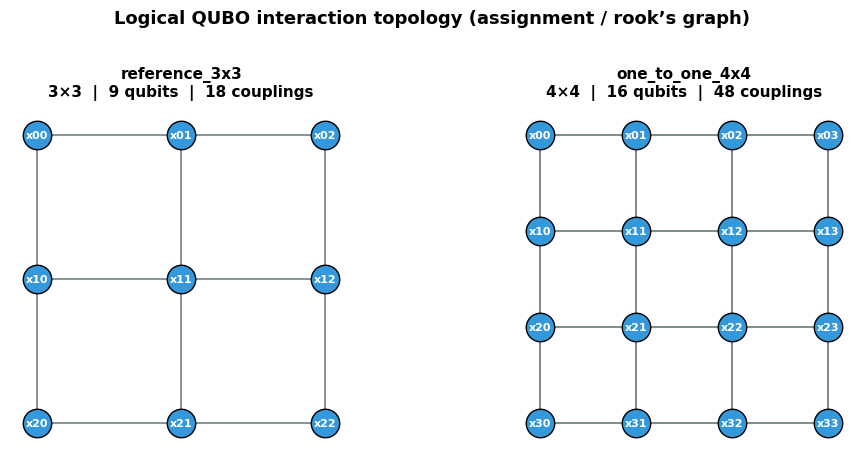
\includegraphics[width=0.92\textwidth]{logical_qubo_topology.png}
\caption{Logical \QUBO{} interaction topology retained from the executed notebook. Row and column cliques create dense couplings before hardware mapping.}
\label{fig:logical_topology}
\end{figure}

\section{Classical Baselines}

The benchmark uses classical solvers on the same matrices and constraints as the quantum workflows. Every solver returns an assignment matrix, score, feasibility flag, runtime, and gap relative to the exact optimum.

\subsection{Exact enumeration}

For the fixed small instances, exact enumeration provides the reference optimum. One-to-one assignments are enumerated as injections or permutations. Exact-capacity assignments are enumerated over resource labels and retained only when their histogram equals $\bm C$. This method is exponential in general but unambiguous for the present validation sizes.

\subsection{Hungarian algorithm}

The Hungarian algorithm solves the square one-to-one linear assignment problem in polynomial time \cite{kuhn1955}. Because the benchmark maximizes affinity, the implementation converts the score matrix to the corresponding minimization form. It is not applied directly to the $4\times2$ exact-capacity representation.

\subsection{Greedy heuristic}

The greedy solver selects high-affinity pairs while respecting the active resource constraints. It is computationally inexpensive but locally myopic; its failure on the $4\times4$ instance is useful as a non-optimal reference.

\subsection{Simulated annealing}

Simulated annealing uses stochastic local updates and an acceptance schedule to explore the assignment space \cite{kirkpatrick1983}. The notebook fixes seed 2026 and evaluates feasibility using the same validation functions as the exact and quantum candidates.

\subsection{Evaluation quantities}

For maximization, the absolute and relative gaps are
\begin{equation}
\absGap=f^\star-f_{\mathrm{best}},
\qquad
\relGap=\frac{f^\star-f_{\mathrm{best}}}{|f^\star|}.
\label{eq:gaps}
\end{equation}
A gap of zero indicates that the best returned feasible assignment equals the exact score. It does not by itself describe sampling concentration or expected energy.

\section{QAOA and GM-QAOA Implementation}

\subsection{Standard QAOA}

Standard \QAOA{} follows the alternating-operator construction introduced by Farhi, Goldstone, and Gutmann \cite{farhi2014} and begins in the uniform superposition
\begin{equation}
\ket{+}^{\otimes N}=H^{\otimes N}\ket{0}^{\otimes N}
\end{equation}
and alternates the penalized cost Hamiltonian $H_Q$ with the transverse-field mixer
\begin{equation}
H_M=\sum_{q=0}^{N-1}X_q.
\end{equation}
At depth $p$, the variational state is
\begin{equation}
\ket{\bm\gamma,\bm\beta}=
\prod_{\ell=1}^{p}
  e^{-i\beta_\ell H_M}
  e^{-i\gamma_\ell H_Q}
\ket{+}^{\otimes N}.
\label{eq:standard_qaoa_state}
\end{equation}
The outer loop minimizes $\langle H_Q\rangle$ with COBYLA. The depth study uses one deterministic initialization and one optimization for each instance--depth pair, rather than a grid search or multi-seed campaign.

\subsection{Grover-Mixer QAOA}

Following the Grover-mixer construction of Bärtschi and Eidenbenz \cite{baertschi2020}, let $\mathcal F$ be the feasible set. \GMQAOA{} assumes a unitary $U_S$ satisfying
\begin{equation}
U_S\ket{0}^{\otimes N}=\ket{F}
=\frac{1}{\sqrt{|\mathcal F|}}
\sum_{x\in\mathcal F}\ket{x}.
\label{eq:feasible_superposition}
\end{equation}
The phase separator is diagonal:
\begin{equation}
U_P(\gamma)=e^{-i\gamma H_C}.
\label{eq:gm_phase_separator}
\end{equation}
Inside $\mathcal F$, every constraint penalty is zero, so the implemented $H_C$ contains only the assignment objective,
\begin{equation}
H_C=-\sum_{i,j}S_{ij}x_{ij}.
\end{equation}
The Grover-like mixer is
\begin{align}
U_M(\beta)
&=e^{-i\beta\ket{F}\!\bra{F}}\\
&=U_S\left[I-\left(1-e^{-i\beta}\right)
\ket{0}\!\bra{0}\right]U_S^\dagger.
\label{eq:grover_mixer}
\end{align}
Consequently, a $p$-round state has the form
\begin{equation}
\ket{\bm\beta,\bm\gamma}=
U_M(\beta_p)U_P(\gamma_p)\cdots
U_M(\beta_1)U_P(\gamma_1)U_S\ket{0}^{\otimes N}.
\end{equation}
The theoretical construction remains inside $\mathcal F$, and equal-quality feasible solutions receive equal amplitudes.

\subsection{Fixed feasible-state preparations}

The Phase-1 implementation constructs exact preparations for three instances:
\begin{itemize}
  \item the uniform superposition of six $3\times3$ permutation matrices;
  \item the uniform superposition of 24 $4\times4$ permutation matrices;
  \item the uniform superposition of six $4\times2$ assignments with two agents per resource.
\end{itemize}
The $4\times2$ preparation creates a weight-two state over the four variables associated with resource 0 and computes the complementary resource-1 variables. Circuit and statevector fidelity are verified against the direct feasible-subspace calculation.

\subsection{Physical realization of the Grover mixer}

For each round, the circuit applies local objective phases, $U_S^\dagger$, $X$ gates on every problem qubit, a multi-controlled phase gate, the inverse $X$ layer, and $U_S$. This directly implements Eq.~\eqref{eq:grover_mixer}; it avoids Trotterization error in the logical mixer. It does not eliminate hardware errors, and the cost of decomposing $U_S$, $U_S^\dagger$, and the multi-controlled phase can be large.

Bärtschi and Eidenbenz give an explicit general permutation preparation with $O(n^3)$ gates and depth $O(n^2)$ on linear-nearest-neighbor architectures \cite{baertschi2020}. The present fixed preparations are exact small-instance constructions, not an implementation of that asymptotic generator. This distinction is maintained throughout the results and compliance analysis.

\section{Experimental Setup}

\subsection{Software environment}

The repository uses the Qiskit software stack \cite{qiskit} and pins Qiskit 2.5.1, Qiskit Aer 0.17.2, Qiskit IBM Runtime 0.48.0, NumPy 2.x, pandas 2.x, SciPy 1.14 or newer, Matplotlib 3.8 or newer, and NetworkX 3.2 or newer. The notebook is designed for sequential execution in Google Colab or an equivalent Python environment. COBYLA is provided through SciPy \cite{virtanen2020}.

The random seed for data generation, statevector sampling, and transpilation is 2026. Standard-\QAOA{} candidate tables use 4096 ideal shots. The hardware comparison uses 1024 shots per circuit.

\subsection{Ideal depth protocol}

Standard \QAOA{} is optimized for
\begin{equation}
p\in\{1,2,3\}
\end{equation}
on all three instances. The original $3\times3$, $p=1$ experiment is retained. No additional parameter grid, multiple optimization seeds, or depth values are introduced. \GMQAOA{} is optimized at $p=1$ for each fixed instance.

\subsection{IBM Quantum execution}

The physical experiment targets the $4\times2$ exact-capacity instance and uses $p=1$ for both algorithms. The archived job metadata are summarized in Table~\ref{tab:job_metadata}.

\begin{table}[H]
\centering
\caption{IBM Quantum job metadata.}
\label{tab:job_metadata}
\begin{tabular}{ll}
\toprule
Field & Recorded value\\
\midrule
Backend & \texttt{ibm\_marrakesh}\\
Backend qubits & 156\\
Job identifier & \texttt{d9vl8qfo3ppc73akfak0}\\
Created (UTC) & 2026-08-14 17:46:17.684431\\
Shots per circuit & 1024\\
Circuits in job & 2\\
Twirling realizations & 16 per circuit\\
Shots per realization & 64\\
Dynamical decoupling & Enabled, XpXm\\
Gate twirling & Enabled\\
Estimated running time & \SI{5.075875}{s}\\
Recorded execution span & \SI{4.400754}{s}\\
Client wall time & \SI{13.695772}{s}\\
\bottomrule
\end{tabular}
\end{table}
The execution span is derived from Runtime timestamps. Client wall time includes submission, service communication, and result retrieval and is not an algorithm-specific QPU duration.

\subsection{Transpilation}

Both measured circuits use the same backend-specific preset pass manager:
\begin{lstlisting}[style=pythonstyle,caption={Backend-specific compilation used in the notebook.}]
pass_manager = generate_preset_pass_manager(
    backend=target_backend,
    optimization_level=3,
    seed_transpiler=2026,
)
standard_isa = pass_manager.run(standard_measured)
gm_isa = pass_manager.run(gm_measured)
\end{lstlisting}
This process selects a physical layout, decomposes non-native gates, and routes interactions through the backend coupling graph. The final native two-qubit operation in the recorded circuits is CZ; the exported CX and ECR counts are zero.

Figure~\ref{fig:topology_overhead} summarizes the logical-to-physical mismatch visible in the executed notebook.
\begin{figure}[H]
\centering
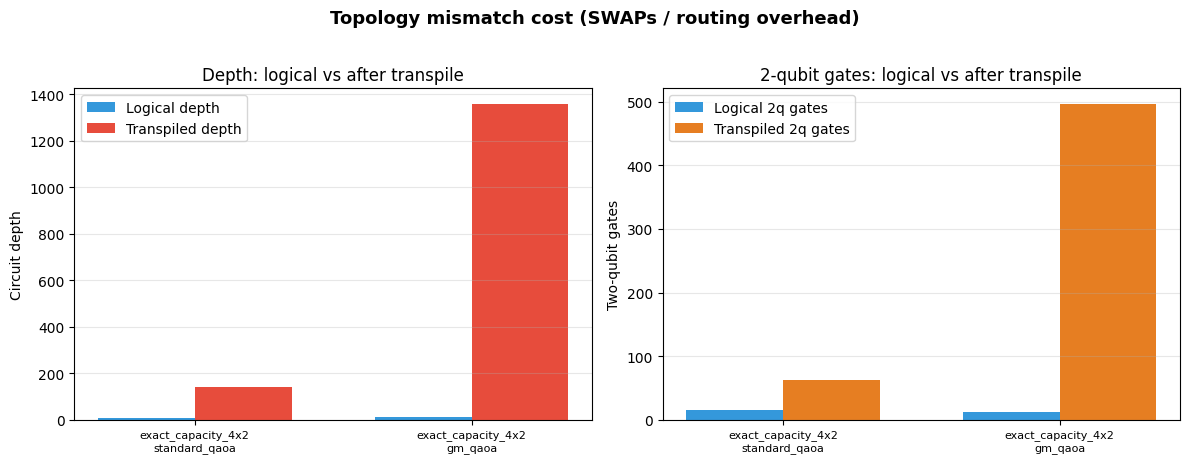
\includegraphics[width=0.98\textwidth]{transpilation_topology_overhead.png}
\caption{Topology and transpilation-overhead summary generated by the executed notebook. Dense logical assignment couplings must be routed on a sparse device graph.}
\label{fig:topology_overhead}
\end{figure}

\subsection{Distribution and uncertainty metrics}

For ideal distribution $p$ and measured distribution $q$,
\begin{align}
\TVD(p,q)&=\frac12\sum_x|p(x)-q(x)|,\label{eq:tvd}\\
\Fcl(p,q)&=\left(\sum_x\sqrt{p(x)q(x)}\right)^2,\label{eq:fidelity}\\
H(p,q)&=\sqrt{1-\sum_x\sqrt{p(x)q(x)}}.
\label{eq:hellinger}
\end{align}
$\Fcl$ is a classical fidelity between measurement distributions, not full quantum-state fidelity on the device. Feasible probability, optimal probability, and leakage are
\begin{equation}
\PF=\sum_{x\in\mathcal F}q(x),
\qquad
\Popt=\sum_{x:f(x)=f^\star}q(x),
\qquad
L_{\mathcal F}=1-\PF.
\end{equation}
Wilson 95\% intervals are used for binomial feasible and optimal counts \cite{wilson1927}.

\subsection{Reconstruction of the complete analysis distribution}

The archived Runtime job contains the complete 1024-shot BitArray for each circuit, from which the full counts are decoded. The \GMQAOA{} ideal distribution is exactly reproduced from its exported $\beta$ and $\gamma$. The repository exports standard-\QAOA{} ideal probabilities to six decimal places but does not retain the full ideal distribution as a separate file. For global standard-\QAOA{} distances, the analytical $p=1$ state is reconstructed by matching those exported probabilities and the exported expected energy, feasible probability, and optimal probability. The recovered values are $\beta\approx1.8352733$ and $\gamma\approx1.2267104$. Standard global distances are therefore reported to four significant digits and identified as reconstructed within the repository's export precision.

\section{Results}

\subsection{Classical baseline results}

Table~\ref{tab:classical_results} reports all classical runs. Exact enumeration and the Hungarian algorithm recover the optimum whenever applicable. Greedy and simulated annealing expose a nontrivial $4\times4$ case: greedy stops at score 2.80, and simulated annealing at 3.01, versus the exact value 3.08.

\begin{table}[H]
\centering
\caption{Classical baseline results exported by the repository.}
\label{tab:classical_results}
\small
\begin{tabular}{llrrr}
\toprule
Instance & Solver & Score & Gap & Runtime (s)\\
\midrule
$3\times3$ & Exact & 2.70 & 0.00 & 0.000466\\
 & Hungarian & 2.70 & 0.00 & 0.000203\\
 & Greedy & 2.70 & 0.00 & 0.003466\\
 & Simulated annealing & 2.70 & 0.00 & 1.909880\\
\midrule
$4\times4$ & Exact & 3.08 & 0.00 & 0.003566\\
 & Hungarian & 3.08 & 0.00 & 0.000151\\
 & Greedy & 2.80 & 0.28 & 0.000417\\
 & Simulated annealing & 3.01 & 0.07 & 2.707101\\
\midrule
$4\times2$, $\bm C=(2,2)$ & Exact & 3.25 & 0.00 & 0.000305\\
 & Greedy & 3.25 & 0.00 & 0.000309\\
 & Simulated annealing & 3.25 & 0.00 & 1.106859\\
\bottomrule
\end{tabular}
\end{table}

These runtimes make clear that the quantum experiment is a correctness and \NISQ{} implementation benchmark, not a runtime competition against classical optimization at this problem size.

\subsection{Standard-QAOA depth comparison}

The ideal depth results are given in Table~\ref{tab:standard_depth}. Bar height in Figure~\ref{fig:depth_comparison} represents feasible probability, while labels report optimal probability.

\begin{table}[H]
\centering
\caption{Ideal standard-\QAOA{} depth sweep.}
\label{tab:standard_depth}
\scriptsize
\resizebox{\textwidth}{!}{%
\begin{tabular}{llrrrrrrr}
\toprule
Instance & $p$ & $\langle Q\rangle$ & $\PF$ (\%) & $\Popt$ (\%) & Best score & Gap & Logical depth & Runtime (s)\\
\midrule
$3\times3$ & 1 & 39.226215 & 0.3583 & 0.0740 & 2.70 & 0.00 & 21 & 1.676498\\
 & 2 & 15.257437 & 8.9024 & 2.1687 & 2.70 & 0.00 & 41 & 1.119079\\
 & 3 & 21.386914 & 11.8618 & 4.1527 & 2.70 & 0.00 & 61 & 1.650187\\
\midrule
$4\times4$ & 1 & 42.062530 & 0.2523 & 0.0029 & 2.80 & 0.28 & 33 & 12.776456\\
 & 2 & 83.253245 & 3.9986 & 0.1629 & 3.08 & 0.00 & 59 & 15.722948\\
 & 3 & 87.475826 & 0.0978 & 0.0092 & 2.80 & 0.28 & 85 & 16.660130\\
\midrule
$4\times2$ & 1 & 18.344321 & 9.1582 & 2.3380 & 3.25 & 0.00 & 21 & 0.297405\\
 & 2 & 8.953983 & 34.8893 & 5.4127 & 3.25 & 0.00 & 38 & 0.358492\\
 & 3 & 7.934315 & 43.9911 & 6.1093 & 3.25 & 0.00 & 55 & 0.452604\\
\bottomrule
\end{tabular}%
}
\end{table}

\begin{figure}[H]
\centering
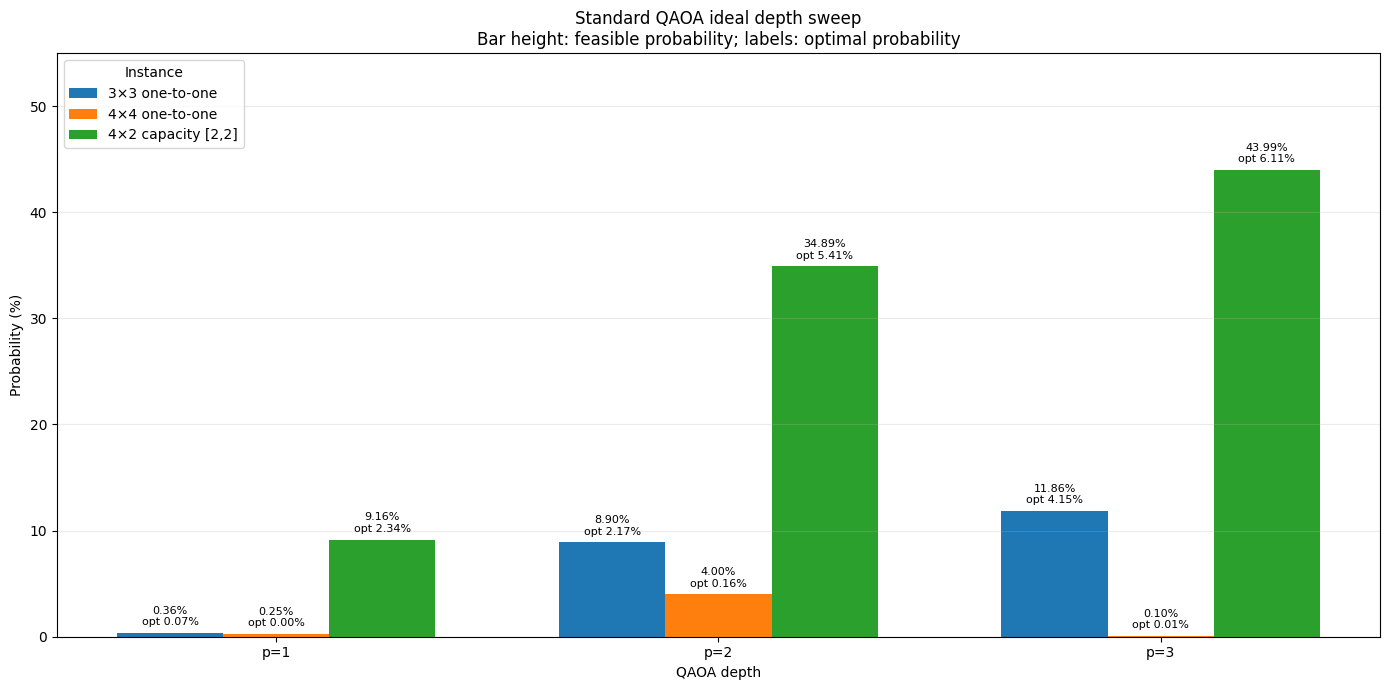
\includegraphics[width=0.98\textwidth]{standard_qaoa_depth_comparison.png}
\caption{Ideal standard-\QAOA{} comparison for $p=1,2,3$. Bar heights show feasible probability and annotations show optimal-solution probability.}
\label{fig:depth_comparison}
\end{figure}

The capacitated $4\times2$ instance shows monotonic gains in $\langle Q\rangle$, $\PF$, and $\Popt$. The $3\times3$ instance increases $\PF$ and $\Popt$ through $p=3$, although its best expected energy occurs at $p=2$. The $4\times4$ instance is non-monotonic: $p=2$ is the only tested depth that samples the optimum, while $p=3$ returns to gap 0.28 and greatly reduces feasible mass. More layers therefore do not guarantee a better optimized state under a fixed optimizer budget.

Figure~\ref{fig:energy_histories} shows the optimization histories for the original $3\times3$ instance.
\begin{figure}[H]
\centering
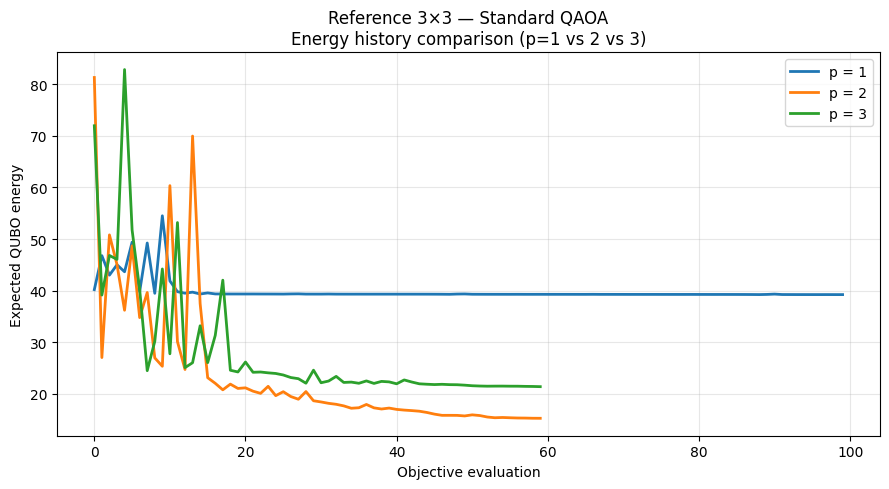
\includegraphics[width=0.82\textwidth]{reference_qaoa_depth_energy_histories.png}
\caption{Expected-\QUBO-energy histories for the reference $3\times3$ standard-\QAOA{} runs.}
\label{fig:energy_histories}
\end{figure}

\subsection{Ideal GM-QAOA results}

Table~\ref{tab:gm_ideal} confirms exact feasible-subspace evolution. State-preparation and full-circuit fidelities are numerically one. All three runs achieve zero best-score gap.

\begin{table}[H]
\centering
\caption{Ideal $p=1$ \GMQAOA{} results.}
\label{tab:gm_ideal}
\scriptsize
\begin{tabular}{lrrrrrrrr}
\toprule
Instance & $\PF$ & $\Popt$ & Best score & Gap & $F(U_S)$ & Circuit fidelity & Depth & Runtime (s)\\
\midrule
$3\times3$ & 1.000000 & 0.692281 & 2.70 & 0.00 & 1.000000 & 1.000000 & 1062 & 0.068595\\
$4\times4$ & 1.000000 & 0.107441 & 3.08 & 0.00 & 1.000000 & 1.000000 & 20252 & 0.059578\\
$4\times2$ & 1.000000 & 0.503666 & 3.25 & 0.00 & 1.000000 & 1.000000 & 395 & 0.086711\\
\bottomrule
\end{tabular}
\end{table}

The ideal probability advantage of \GMQAOA{} is pronounced on the fixed cases, but the decomposed depths reveal the state-preparation cost. In particular, the $4\times4$ fixed construction has depth 20252 before any hardware routing experiment and was therefore not selected for QPU execution.

\subsection{IBM Quantum results}

The hardware experiment includes only the $4\times2$ instance and $p=1$. Table~\ref{tab:hardware_quality} distinguishes best-sample quality from distribution concentration.

\begin{table}[H]
\centering
\caption{Hardware quality for the exact-capacity $4\times2$ instance.}
\label{tab:hardware_quality}
\small
\begin{tabular}{lrrrrrr}
\toprule
Algorithm & Shots & Minimum $Q$ & Best score & Gap & $\PF$ & $\Popt$\\
\midrule
Standard \QAOA{} & 1024 & $-3.25$ & 3.25 & 0.00 & 0.077148 & 0.015625\\
\GMQAOA{} & 1024 & $-3.25$ & 3.25 & 0.00 & 0.119141 & 0.028320\\
\bottomrule
\end{tabular}
\end{table}

Both distributions contain \texttt{10011001}, the exact optimum. The most frequently observed standard-\QAOA{} state is instead infeasible \texttt{10101101} with 23 counts. In \GMQAOA{}, the optimal state is the modal output with 29 counts, but the remaining probability is distributed broadly and mostly outside the feasible set.

\subsection{Transpilation and resource overhead}

\begin{table}[H]
\centering
\caption{Logical and transpiled resource counts on \texttt{ibm\_marrakesh}.}
\label{tab:transpilation}
\small
\resizebox{\textwidth}{!}{%
\begin{tabular}{lrrrrrrrr}
\toprule
Algorithm & Depth before & Depth after & Size before & Size after & 2Q before & 2Q after & CZ & Transpile (s)\\
\midrule
Standard \QAOA{} & 10 & 143 & 48 & 293 & 16 & 63 & 63 & 0.023831\\
\GMQAOA{} & 11 & 1357 & 60 & 2180 & 12 & 496 & 496 & 0.132162\\
\bottomrule
\end{tabular}%
}
\end{table}

Relative to standard \QAOA{}, the physical \GMQAOA{} circuit has $9.49\times$ the depth, $7.44\times$ the number of instructions, and $7.87\times$ the native two-qubit gates. Relative to its own abstract circuit, \GMQAOA{} experiences $123.36\times$ depth inflation, compared with $14.3\times$ for standard \QAOA{}.

\begin{figure}[H]
\centering
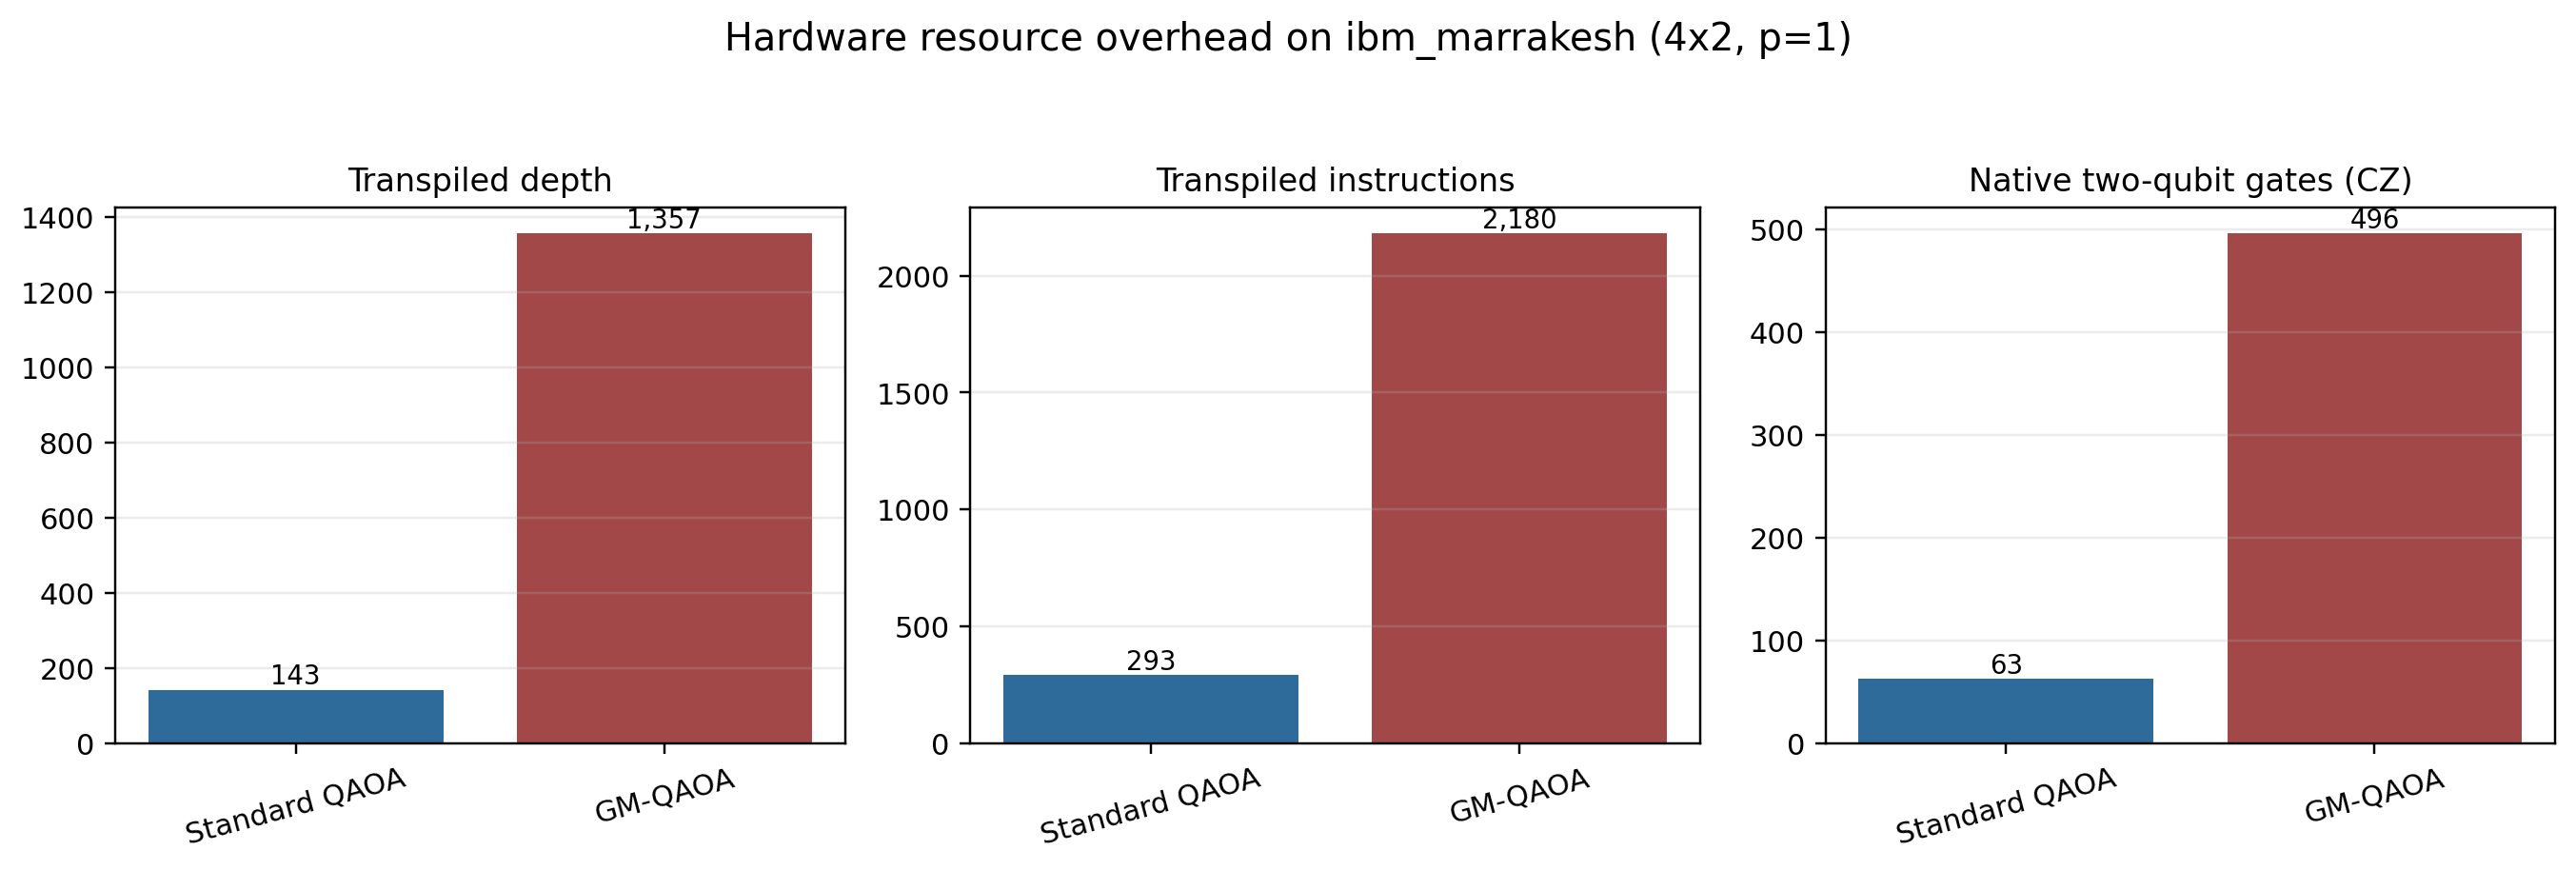
\includegraphics[width=0.98\textwidth]{hardware_resource_overhead.png}
\caption{Transpiled resource overhead for the two circuits executed in the same Runtime job.}
\label{fig:resource_overhead}
\end{figure}

\section{Error Analysis and Noise Characterization}

\subsection{Ideal versus hardware distributions}

Figure~\ref{fig:ideal_hardware_hist} is the wide histogram generated in the executed notebook. It compares a 1024-shot ideal reference with the measured \texttt{ibm\_marrakesh} counts on the same selected support. The standard distribution is moderately distorted. The \GMQAOA{} distribution exhibits a much larger collapse of the dominant ideal peaks and substantial population of states having zero ideal probability.

\begin{figure}[H]
\centering
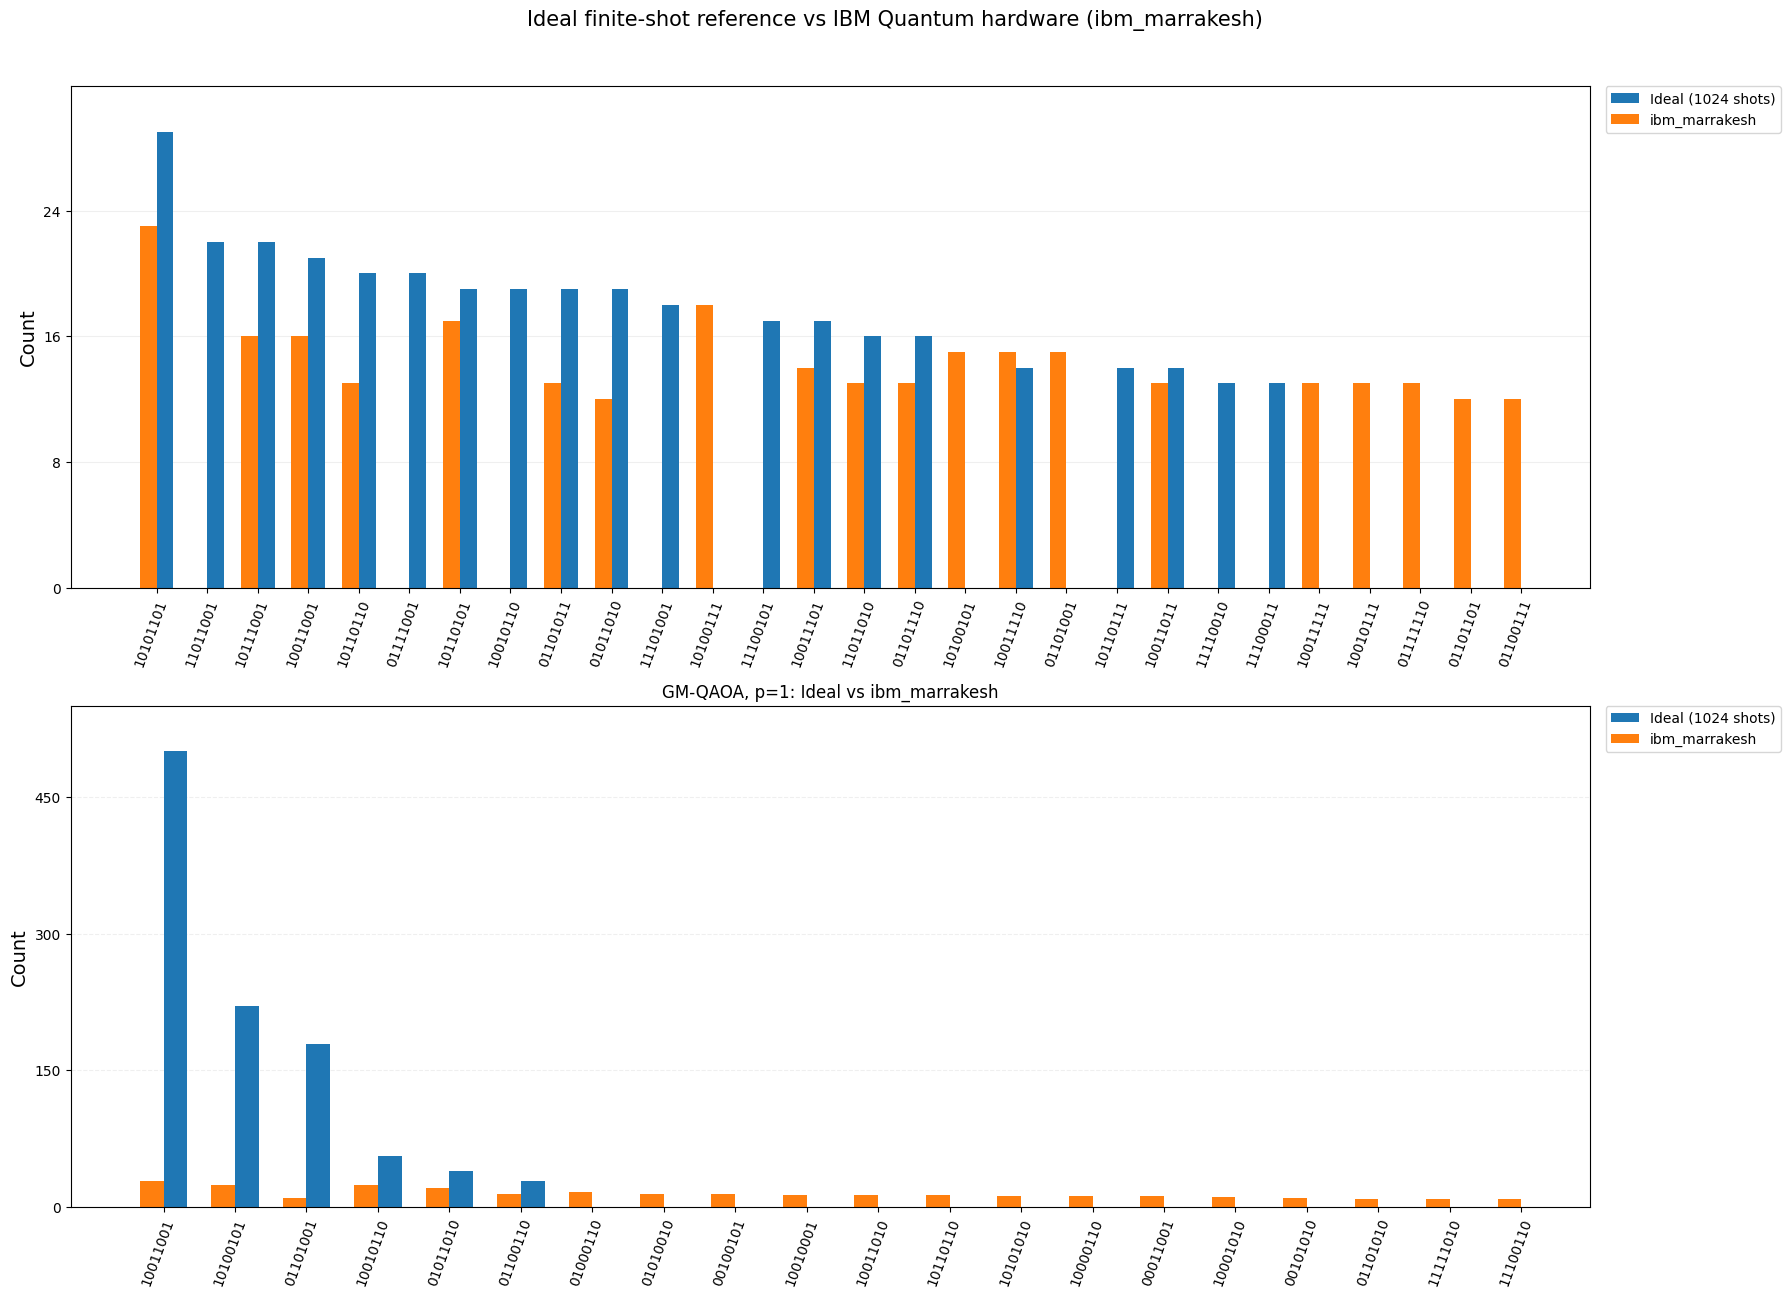
\includegraphics[width=0.99\textwidth]{ideal_vs_ibm_marrakesh_histograms.png}
\caption{Ideal finite-shot reference versus IBM Quantum hardware for standard \QAOA{} and \GMQAOA{}. The bottom panel makes the collapse of the ideal \GMQAOA{} peaks visible.}
\label{fig:ideal_hardware_hist}
\end{figure}

\subsection{Feasible and optimal probabilities}

Table~\ref{tab:probability_degradation} compares exact ideal values with complete hardware counts. The standard ideal values and its global distribution metrics are reconstructed within the six-decimal precision of the repository exports, as explained in Section~6.

\begin{table}[H]
\centering
\caption{Ideal-to-hardware probability degradation.}
\label{tab:probability_degradation}
\small
\begin{tabular}{lrrrrrr}
\toprule
Algorithm & Ideal $\PF$ & QPU $\PF$ & Ideal $\Popt$ & QPU $\Popt$ & $\Delta\Popt$ & Relative $\Popt$ error\\
\midrule
Standard \QAOA{} & 0.091582 & 0.077148 & 0.023380 & 0.015625 & $-0.007755$ & $-33.17\%$\\
\GMQAOA{} & 1.000000 & 0.119141 & 0.503666 & 0.028320 & $-0.475346$ & $-94.38\%$\\
\bottomrule
\end{tabular}
\end{table}

\begin{figure}[H]
\centering
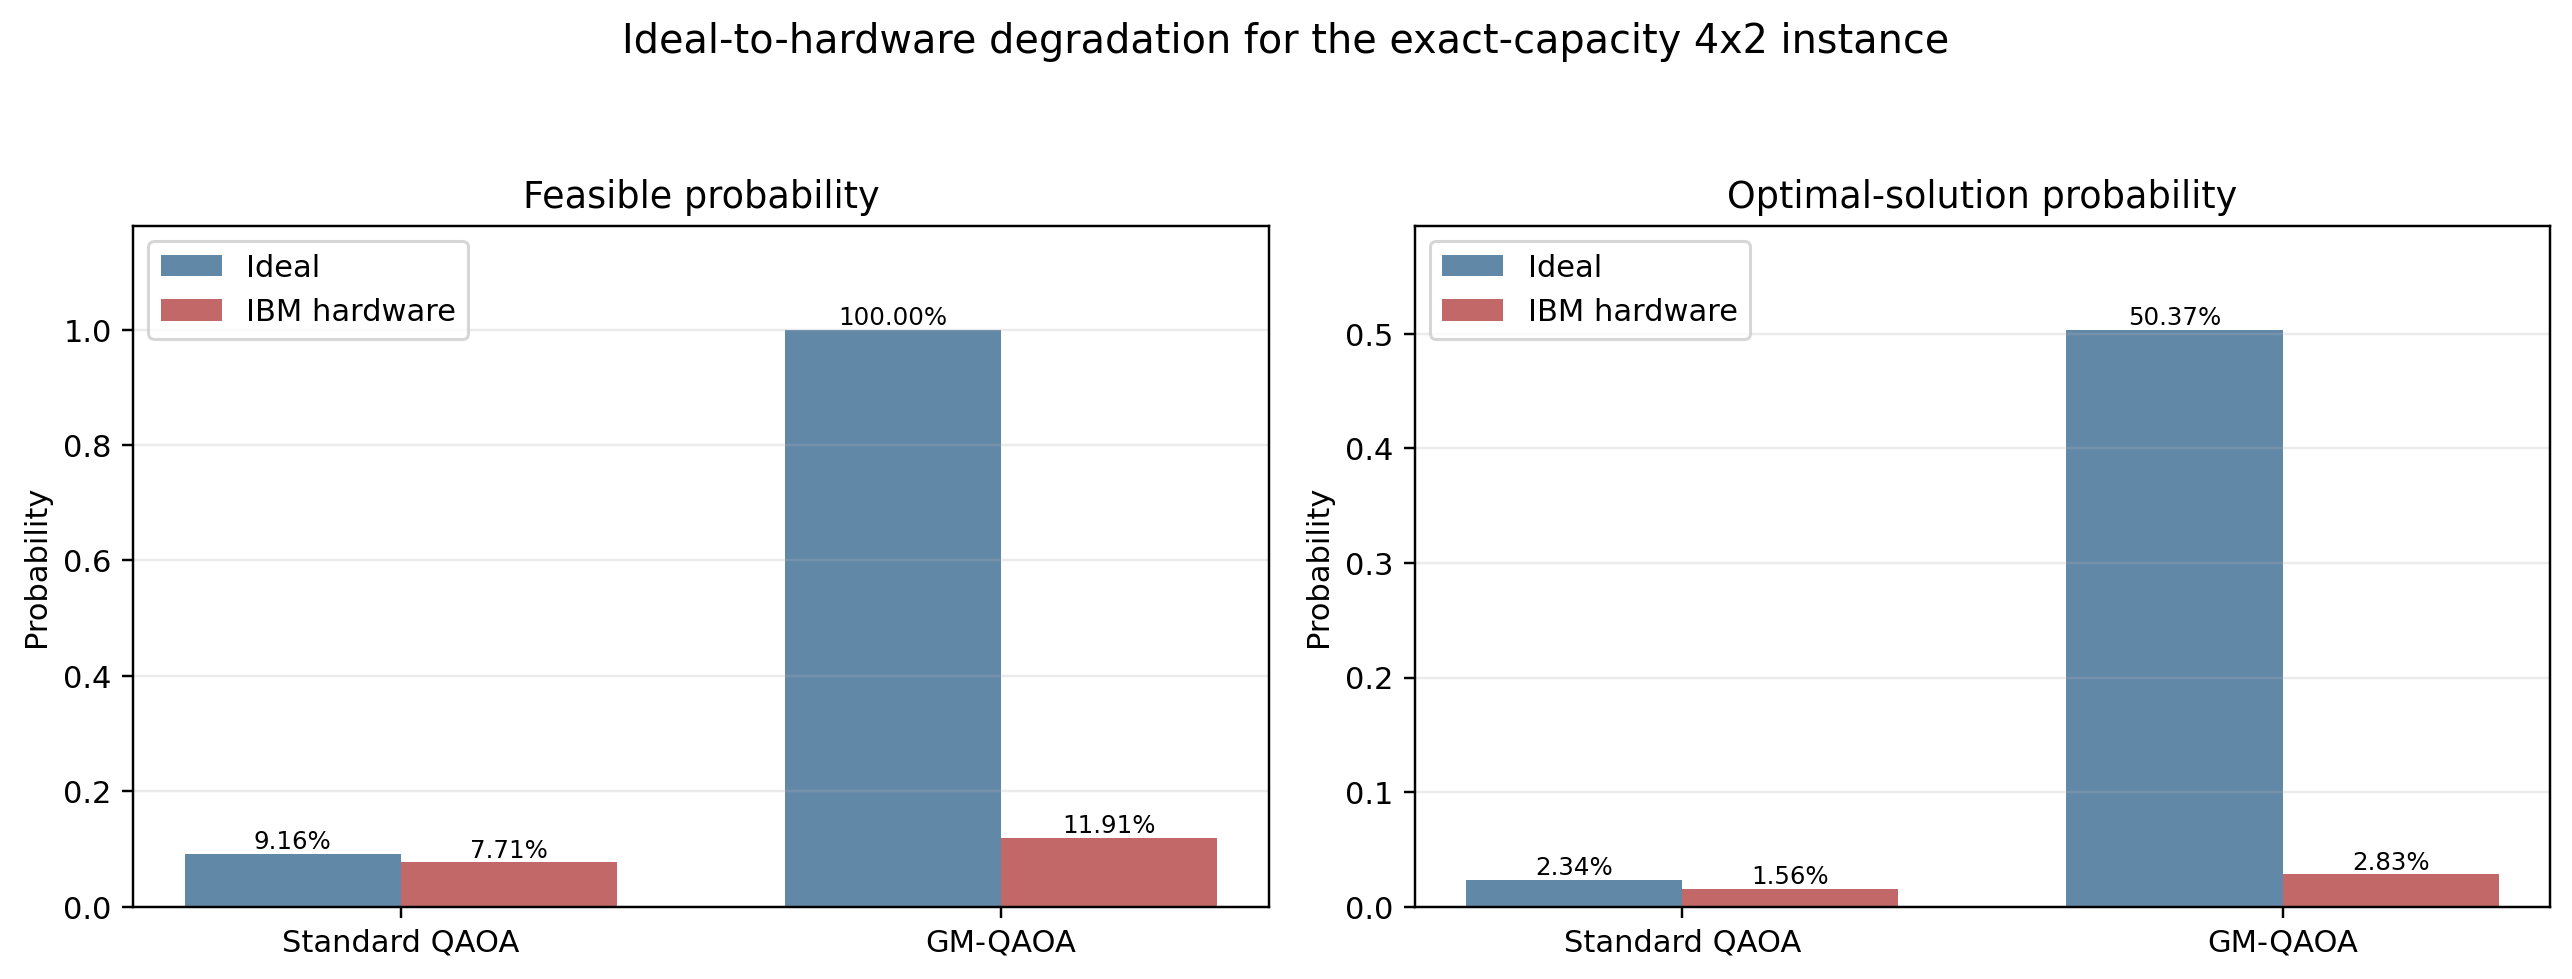
\includegraphics[width=0.96\textwidth]{ideal_hardware_quality_comparison.png}
\caption{Ideal and physical feasible/optimal probabilities for the hardware instance.}
\label{fig:quality_comparison}
\end{figure}

The 95\% Wilson intervals are
\begin{align}
P_{\mathrm{F,QPU}}^{\mathrm{std}}&\in[0.06234,0.09512],&
P_{\mathrm{opt,QPU}}^{\mathrm{std}}&\in[0.00964,0.02523],\\
P_{\mathrm{F,QPU}}^{\mathrm{GM}}&\in[0.10071,0.14042],&
P_{\mathrm{opt,QPU}}^{\mathrm{GM}}&\in[0.01979,0.04038].
\end{align}
The standard ideal optimum probability lies inside its physical interval, whereas the \GMQAOA{} ideal optimum probability is far outside the physical interval.

\subsection{Global distribution metrics}

\begin{table}[H]
\centering
\caption{Distribution-level errors. Standard values marked $\dagger$ are reconstructed within the precision of the exported ideal probabilities.}
\label{tab:distribution_metrics}
\begin{tabular}{lrrrr}
\toprule
Algorithm & TVD & Hellinger & $\Fcl$ & $1-\TVD$\\
\midrule
Standard \QAOA{}$^\dagger$ & 0.2082 & 0.2346 & 0.8929 & 0.7918\\
\GMQAOA{} & 0.8809 & 0.8284 & 0.0984 & 0.1191\\
\bottomrule
\end{tabular}
\end{table}

\begin{figure}[H]
\centering
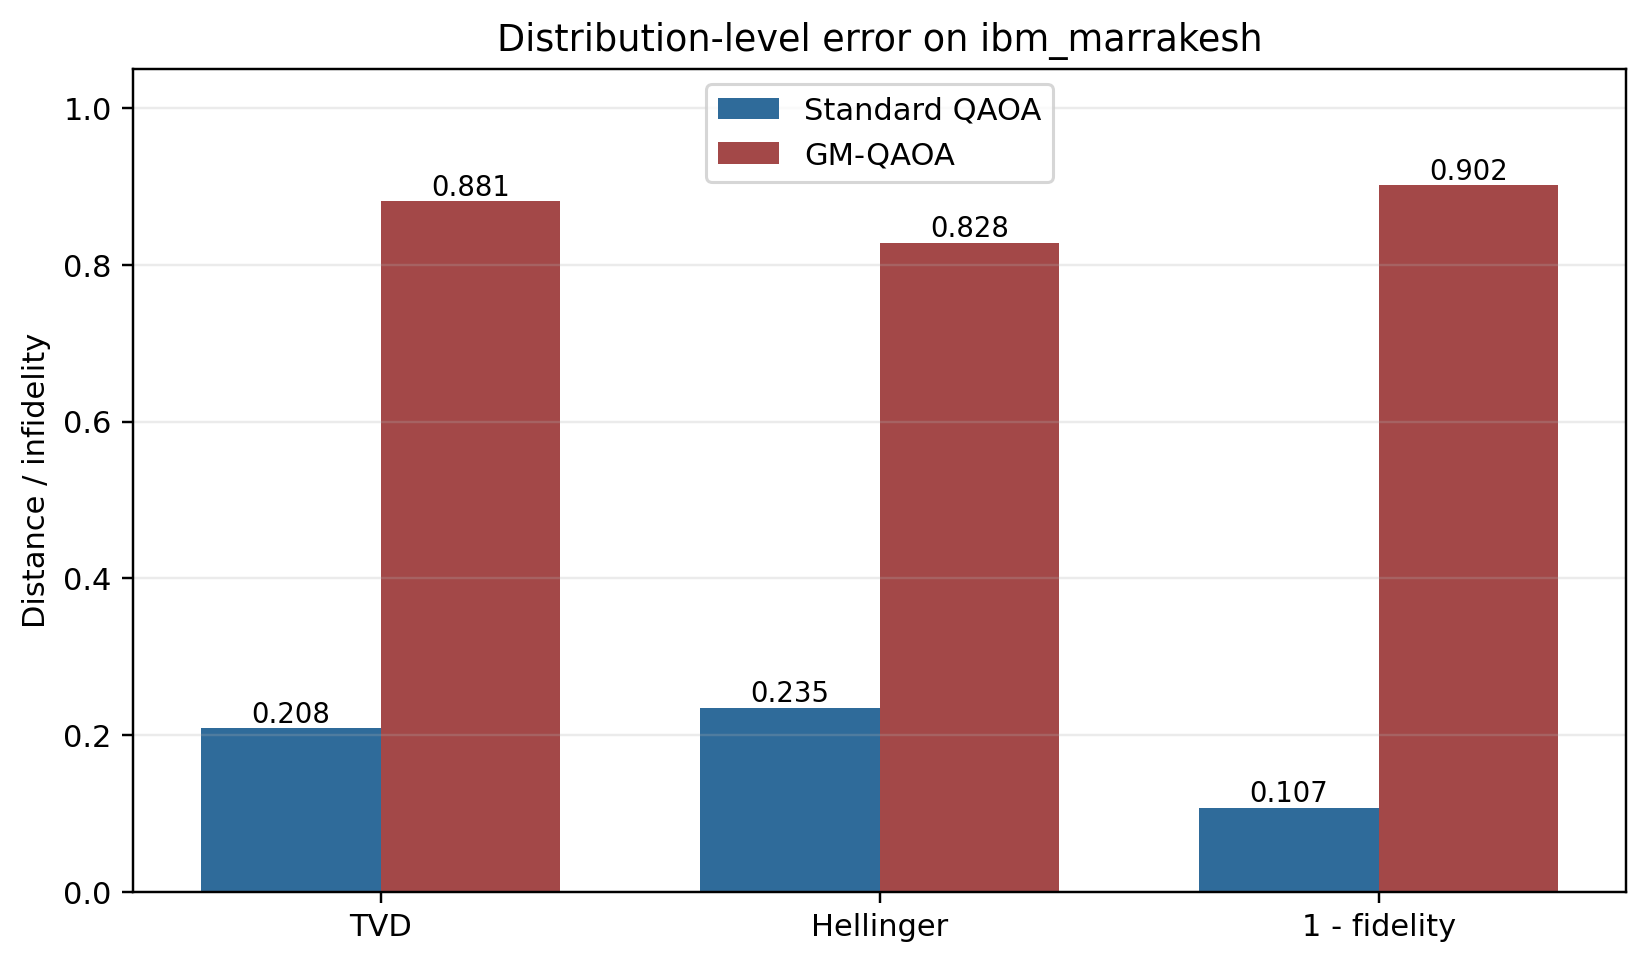
\includegraphics[width=0.76\textwidth]{distribution_error_metrics.png}
\caption{Distribution-level distance and infidelity measures derived from the complete archived counts.}
\label{fig:error_metrics}
\end{figure}

For \GMQAOA{}, the ideal distribution has support only on $\mathcal F$. All six measured feasible probabilities remain below their ideal values, so the TVD equals the measured leakage:
\begin{equation}
\TVD_{\mathrm{GM}}=1-P_{\mathrm{F,QPU}}^{\mathrm{GM}}=0.880859375.
\end{equation}
This equality provides a direct interpretation of the error: $88.09\%$ of measured probability has leaked outside the ideal support.

\subsection{Energy distortion}

The expected penalized energies change as follows:
\begin{table}[H]
\centering
\caption{Ideal and observed expected \QUBO{} energies.}
\label{tab:energy_distortion}
\begin{tabular}{lrrr}
\toprule
Algorithm & Ideal $\langle Q\rangle$ & QPU $\langle Q\rangle$ & Difference\\
\midrule
Standard \QAOA{}$^\dagger$ & 18.3443 & 19.6276 & $+1.2833$\\
\GMQAOA{} & $-2.8453$ & 20.2492 & $+23.0945$\\
\bottomrule
\end{tabular}
\end{table}
The \GMQAOA{} expected energy loses the advantage implied by its ideal feasible-state concentration, even though one optimal sample remains visible.

\subsection{Noise mechanisms and evidence}

The experiment does not isolate a single microscopic error channel. The observed distortion is consistent with the combined effects of:
\begin{itemize}
  \item synthesis of controlled state preparations and the multi-controlled phase;
  \item routing on a sparse coupling graph;
  \item accumulated CZ and single-qubit gate error;
  \item decoherence during a substantially longer schedule;
  \item measurement error;
  \item calibration drift and stochastic variation across twirling realizations.
\end{itemize}
Dynamical decoupling and gate twirling were enabled, so the results already include those suppression techniques. Their presence does not constitute a no-mitigation control experiment. The resource contrast strongly supports circuit length as a major explanatory factor, but it does not prove that depth alone caused the observed difference.

\subsection{Best-sample error versus statistical reliability}

Both algorithms have zero best-sample optimization gap because the optimum appeared at least once. This statement is compatible with low reliability: the optimal state occurred only 16 times for standard \QAOA{} and 29 times for \GMQAOA{} out of 1024 shots. A publication claim should therefore report the gap jointly with $\Popt$, confidence intervals, $\PF$, and global distances.

\section{Discussion and Limitations}

\subsection{Depth is instance- and metric-dependent}

The ideal standard-\QAOA{} sweep does not support a universal claim that larger $p$ improves performance. For the $4\times2$ instance, $p=3$ is best under expected energy, feasible probability, and optimal probability. For $3\times3$, $p=2$ has the lowest expected energy while $p=3$ has higher feasible and optimal probabilities. For $4\times4$, the tested $p=3$ run is worse than $p=2$ and fails to recover the optimum. Optimization budget, initialization, and landscape structure interact with depth.

\subsection{GM-QAOA shifts rather than removes complexity}

In ideal simulation, \GMQAOA{} offers a clean separation between feasibility and optimization. Penalty terms are unnecessary inside $\mathcal F$, feasible probability is exactly one, and the optimum receives substantially more probability than under standard \QAOA{} at $p=1$. The hardware result shows the trade-off emphasized by Bärtschi and Eidenbenz: the approach is useful only when $U_S$ and its inverse can be compiled efficiently \cite{baertschi2020}.

For the compact $4\times2$ case, the physical Grover-mixer circuit is nearly ten times deeper and contains nearly eight times as many native two-qubit gates as the standard circuit. Its ideal $50.37\%$ optimum probability collapses to $2.83\%$. Thus, feasible-subspace design at the logical level is not sufficient; state-preparation architecture and device-aware synthesis determine whether the theoretical benefit survives.

\subsection{Alignment with QI26-20}

The artifact fulfills the central implementation path of QI26-20: synthetic assignment data, one-to-one and one-to-$N$ constraints, \QUBO{} formulation, classical baselines, ideal \QAOA{}, real IBM Quantum execution, and analysis of depth and noise-related overhead \cite{qi2620}. It also preserves the depth supplement's restricted $p=1,2,3$ experiment \cite{depthsupplement}. A complete six-week research program would additionally require a systematic size family, broader tuning, and repeated physical experiments.

\subsection{Alignment with Bärtschi and Eidenbenz}

The notebook implements the operational equations
\begin{equation}
U_S\ket{0}=\ket{F},\qquad
U_P(\gamma)=e^{-i\gamma H_C},\qquad
U_M(\beta)=U_SD_0(\beta)U_S^\dagger
\end{equation}
and verifies ideal feasible-subspace preservation. It does not implement the paper's general permutation generator or demonstrate its asymptotic complexity. The absence of Hamiltonian-simulation error in the logical mixer must not be confused with absence of physical noise.

\subsection{Threats to validity}

The main limitations are:
\begin{enumerate}
  \item \textbf{Small fixed instances.} Eight, nine, and sixteen logical qubits do not establish scaling behavior.
  \item \textbf{Single deterministic optimization.} No optimizer-seed variance or parameter-sensitivity distribution is measured.
  \item \textbf{One physical job.} The study cannot estimate temporal drift or between-job variance.
  \item \textbf{One backend.} Results are not portable to other topologies or calibration regimes without new transpilation and execution.
  \item \textbf{Hardware depth restricted to $p=1$.} The ideal $p=2,3$ conclusions are not physical results.
  \item \textbf{Fixed feasible-state preparations.} They are exact demonstrations, not a general scalable library.
  \item \textbf{No ablation study.} Dynamical decoupling and twirling are enabled, but there are no matched controls without these options.
  \item \textbf{Standard global metric reconstruction.} Standard ideal-to-hardware distances use a distribution reconstructed within the six-decimal precision of repository exports; the complete ideal vector should be exported directly in future releases.
\end{enumerate}

\subsection{No quantum-advantage claim}

Exact and Hungarian solvers obtain the optimum orders of magnitude faster than the quantum workflow at these sizes. The reported contribution is a reproducible formulation and hardware-error benchmark. Neither runtime advantage nor solution-quality advantage over appropriate classical algorithms is demonstrated.

\section{Conclusion and Future Work}

This study delivers a traceable \QUBO--\QAOA{} benchmark for generalized bipartite assignment. The formulation supports one-to-one assignment and fixed exact capacities, and its \QUBO-to-Ising mapping is numerically validated. Four classical baselines, a standard-\QAOA{} depth sweep, ideal \GMQAOA{}, backend-specific transpilation, and a real IBM Quantum comparison are integrated in one repository artifact.

The ideal standard-\QAOA{} study shows that the effect of depth is not monotonic across instances. The exact-capacity $4\times2$ case benefits consistently through $p=3$, while the $4\times4$ case is best at $p=2$ under the tested settings. Ideal \GMQAOA{} preserves the feasible subspace and yields zero best-score gap for all three fixed instances.

On \texttt{ibm\_marrakesh}, both $p=1$ algorithms sampled the exact optimum. Nevertheless, standard \QAOA{} retained a distribution much closer to its ideal reference than \GMQAOA{}. The Grover-mixer circuit incurred depth 1357 and 496 CZ gates, versus depth 143 and 63 CZ gates for standard \QAOA{}. Its feasible mass fell from $100\%$ to $11.91\%$, and its optimal probability from $50.37\%$ to $2.83\%$. The primary scientific conclusion is therefore not that \GMQAOA{} fails as an ideal ansatz, but that the specific fixed feasible-state preparation and selective-phase implementation are too costly to preserve their ideal advantage on this hardware execution.

Future work should:
\begin{enumerate}
  \item export complete ideal and measured distributions directly with every run;
  \item repeat matched jobs across time and backends, with uncertainty over calibrations;
  \item evaluate hardware $p=2,3$ only after resource preflight;
  \item replace generic or controlled state preparations with structured $W$/Dicke, bitmask, swap, and ancilla-reuse constructions;
  \item compare alternative multi-controlled-phase syntheses and layouts;
  \item perform ablations for readout mitigation, dynamical decoupling, twirling, and postselection;
  \item construct a controlled family of instance sizes and capacity vectors;
  \item report total resource cost jointly with solution quality and classical baselines.
\end{enumerate}

Within its stated scope, the artifact satisfies the intended Phase-1 objective: it converts a student-developed assignment benchmark into a reproducible research workflow with explicit theoretical alignment, real-hardware evidence, error analysis, and clearly bounded claims.


\section*{Author Contributions}
\addcontentsline{toc}{section}{Author Contributions}
The contribution statement follows the ownership recorded in the notebook. Jiya Maurya led the mathematical formulation and \QUBO{} derivation, with support from Satkar Juneja and Ilia Fazeli. Abhishek Raj led synthetic-data generation and constraint validation, with support from Jiya Maurya and Satkar Juneja. Satkar Juneja led the classical baselines and evaluation metrics, with support from Jiya Maurya and Marcos Jiménez. Marcos Jiménez led the Qiskit/\QAOA{} simulator implementation, with support from Ilia Fazeli, Abhishek Raj, and Satkar Juneja. Ilia Fazeli led documentation and experiment tracking, with support from Marcos Jiménez and Jiya Maurya. Iván Barrientos Salas provided conceptualization, supervision, scientific auditing, integration of generalized capacities and \GMQAOA{}, hardware methodology, validation, and manuscript preparation. All authors should confirm the final CRediT taxonomy and author order before journal submission.

\section*{Data and Code Availability}
\addcontentsline{toc}{section}{Data and Code Availability}
The reproducible artifact is organized as the repository \texttt{QI26-20-QUBO-QAOA-Benchmark}. It contains the executed notebook, dependency specification, exported result tables, scientific-claims checklist, and compliance matrix. The archived IBM Quantum job identifier is \texttt{d9vl8qfo3ppc73akfak0}. The public repository URL should be inserted when the repository is released. The full distribution table reconstructed from the archived Runtime result is included with the manuscript source under \texttt{Data/full\_hardware\_distributions.csv}.

\section*{Acknowledgments}
\addcontentsline{toc}{section}{Acknowledgments}
This work was developed in the QI26-20 / QIntern 2026 research context. The authors acknowledge the use of Qiskit and IBM Quantum services. Access to the quantum processing unit does not imply endorsement of the conclusions by IBM.

\section*{Funding and Conflicts of Interest}
\addcontentsline{toc}{section}{Funding and Conflicts of Interest}
Funding and conflict-of-interest declarations were not specified in the repository artifacts and must be confirmed by all authors before external submission.

\clearpage
\appendix
\section{Compliance Matrix}
\label{app:compliance}

\begin{landscape}
\small
\setlength{\tabcolsep}{4pt}
\begin{longtable}{p{0.14\linewidth}p{0.28\linewidth}p{0.14\linewidth}p{0.38\linewidth}}
\caption{Formal compliance with QI26-20, the depth supplement, and Bärtschi--Eidenbenz.}\\
\toprule
Reference & Requirement & Status & Evidence and reservation\\
\midrule
\endfirsthead
\toprule
Reference & Requirement & Status & Evidence and reservation\\
\midrule
\endhead
Depth supplement & Preserve original $3\times3$, $p=1$ experiment & \cellcolor{AuditMet}\textbf{Met} & The reference run remains explicit and uses the original initialization and analysis aliases.\\
Depth supplement & Add $4\times4$ one-to-one instance & \cellcolor{AuditMet}\textbf{Met} & Reproducible seed-2026 affinity matrix and exact one-to-one constraints.\\
Depth supplement & Add $4\times2$ capacities $[2,2]$ & \cellcolor{AuditMet}\textbf{Met} & Exact squared capacity penalty and direct feasibility validation.\\
Depth supplement & Standard-\QAOA{} sweep $p=1,2,3$ & \cellcolor{AuditMet}\textbf{Met ideally} & Nine deterministic statevector experiments; no additional depth grid.\\
QI26-20 & Classical baselines and same-instance comparison & \cellcolor{AuditMet}\textbf{Met} & Exact, Hungarian, greedy, and simulated annealing use the same matrices and score definitions.\\
QI26-20 & Real hardware execution & \cellcolor{AuditMet}\textbf{Met for fixed case} & Standard \QAOA{} and \GMQAOA{} executed on \texttt{ibm\_marrakesh}, job \texttt{d9vl8qfo3ppc73akfak0}.\\
QI26-20 & Depth, noise, and resource analysis & \cellcolor{AuditPartial}\textbf{Partial} & Ideal depth sweep and $p=1$ QPU resource/error analysis are present; no QPU $p=2,3$ campaign.\\
QI26-20 & Scaling over increasing graph sizes & \cellcolor{AuditPartial}\textbf{Partial} & Three sizes are represented, but no systematic scaling regression or broad family.\\
Bärtschi--Eidenbenz & Equal feasible-state superposition & \cellcolor{AuditMet}\textbf{Met for fixed cases} & State-preparation fidelity equals one in ideal simulation.\\
Bärtschi--Eidenbenz & Parameterized Grover mixer & \cellcolor{AuditMet}\textbf{Met operationally} & $U_SD_0(\beta)U_S^\dagger$ is implemented with a selective phase.\\
Bärtschi--Eidenbenz & Ideal feasible-subspace preservation & \cellcolor{AuditMet}\textbf{Met ideally} & $\PF=1$ and full-circuit state fidelity equals one for all fixed cases.\\
Bärtschi--Eidenbenz & General $O(n^3)$ permutation preparation & \cellcolor{AuditNo}\textbf{Not implemented} & Phase 1 uses exact fixed-size constructions and makes no general asymptotic claim.\\
Scientific claim & Quantum advantage & \cellcolor{AuditNo}\textbf{Not established} & Classical exact and Hungarian methods dominate these small instances; one hardware job is insufficient.\\
\bottomrule
\end{longtable}
\end{landscape}

\clearpage
\begin{landscape}
\section{Transpiled Circuit Views}
\label{app:circuits}

The complete folded standard-\QAOA{} ISA circuit is shown in Figure~\ref{fig:std_folded}. Idle physical wires are omitted by the notebook drawer. The \GMQAOA{} circuit is substantially taller in folded form, so it is split into four overlapping panels. The full original image is retained as \path{Figures/gm_qaoa_transpiled_folded_full.png} in the source package.

\begin{figure}[H]
\centering
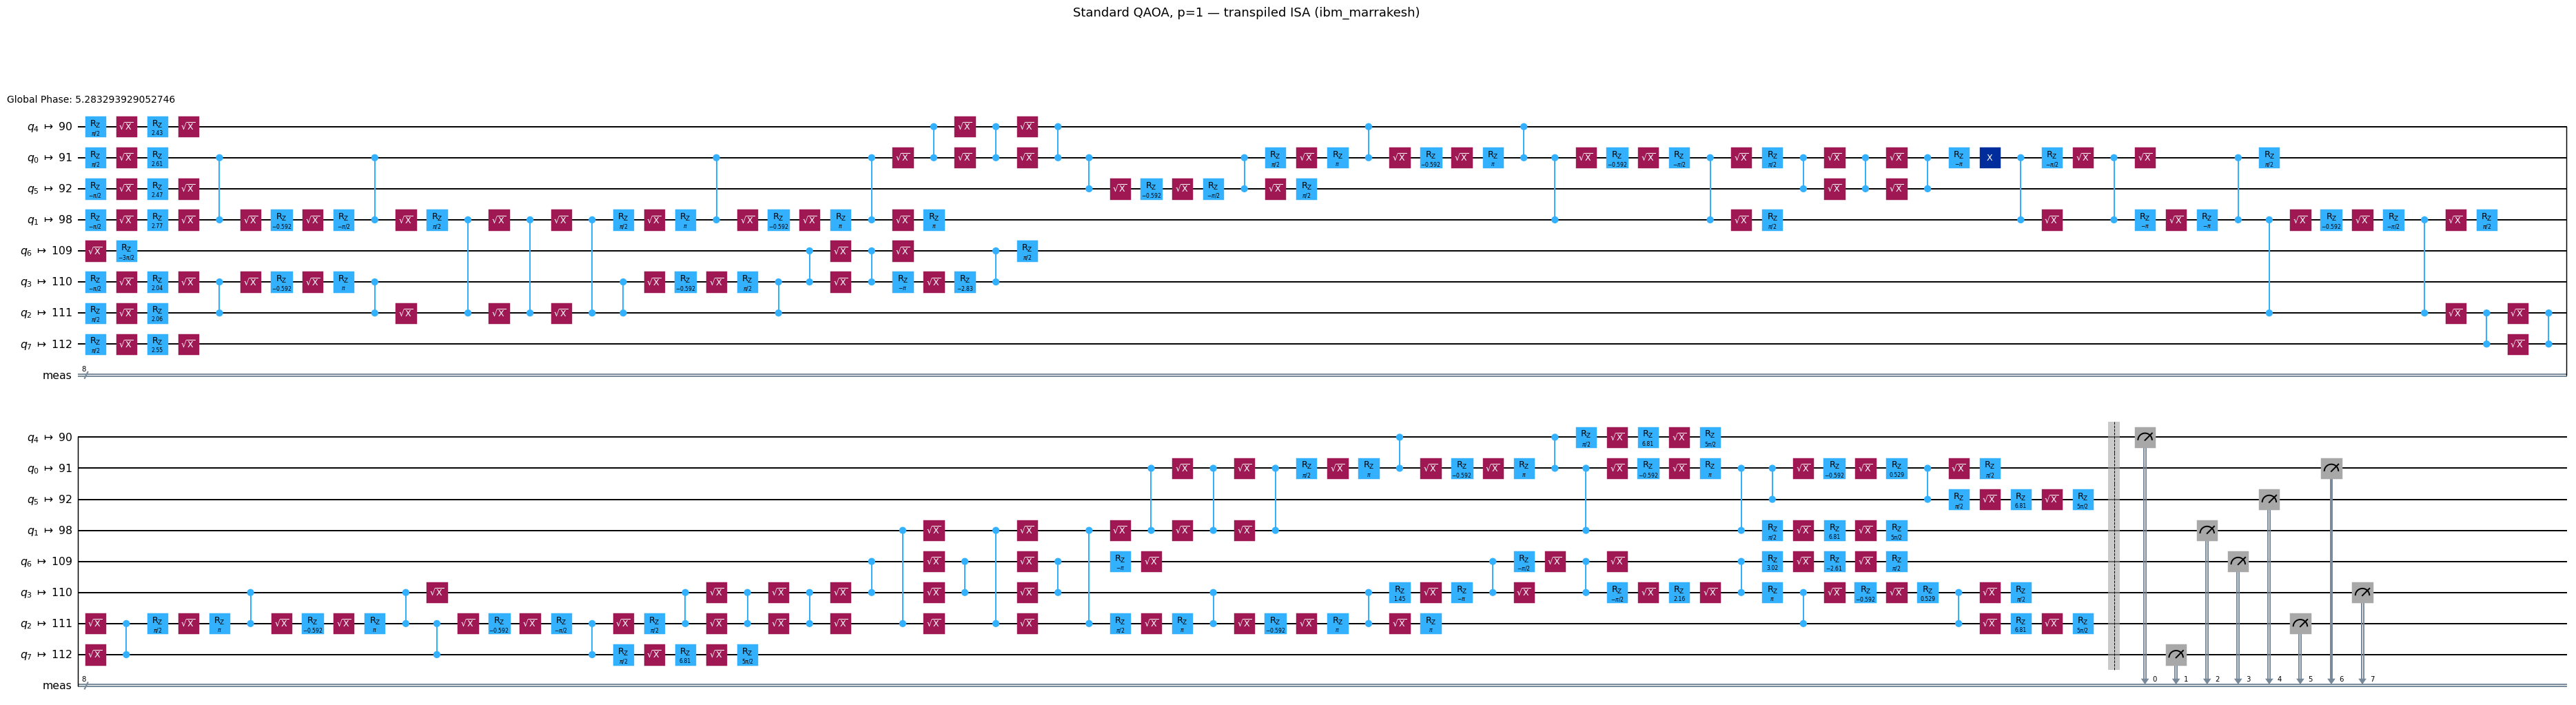
\includegraphics[width=0.98\linewidth,height=0.58\textheight,keepaspectratio]{standard_qaoa_transpiled_folded.png}
\caption{Standard-\QAOA{} $p=1$ circuit after transpilation to \texttt{ibm\_marrakesh}.}
\label{fig:std_folded}
\end{figure}
\end{landscape}

\begin{landscape}
\begin{figure}[H]
\centering
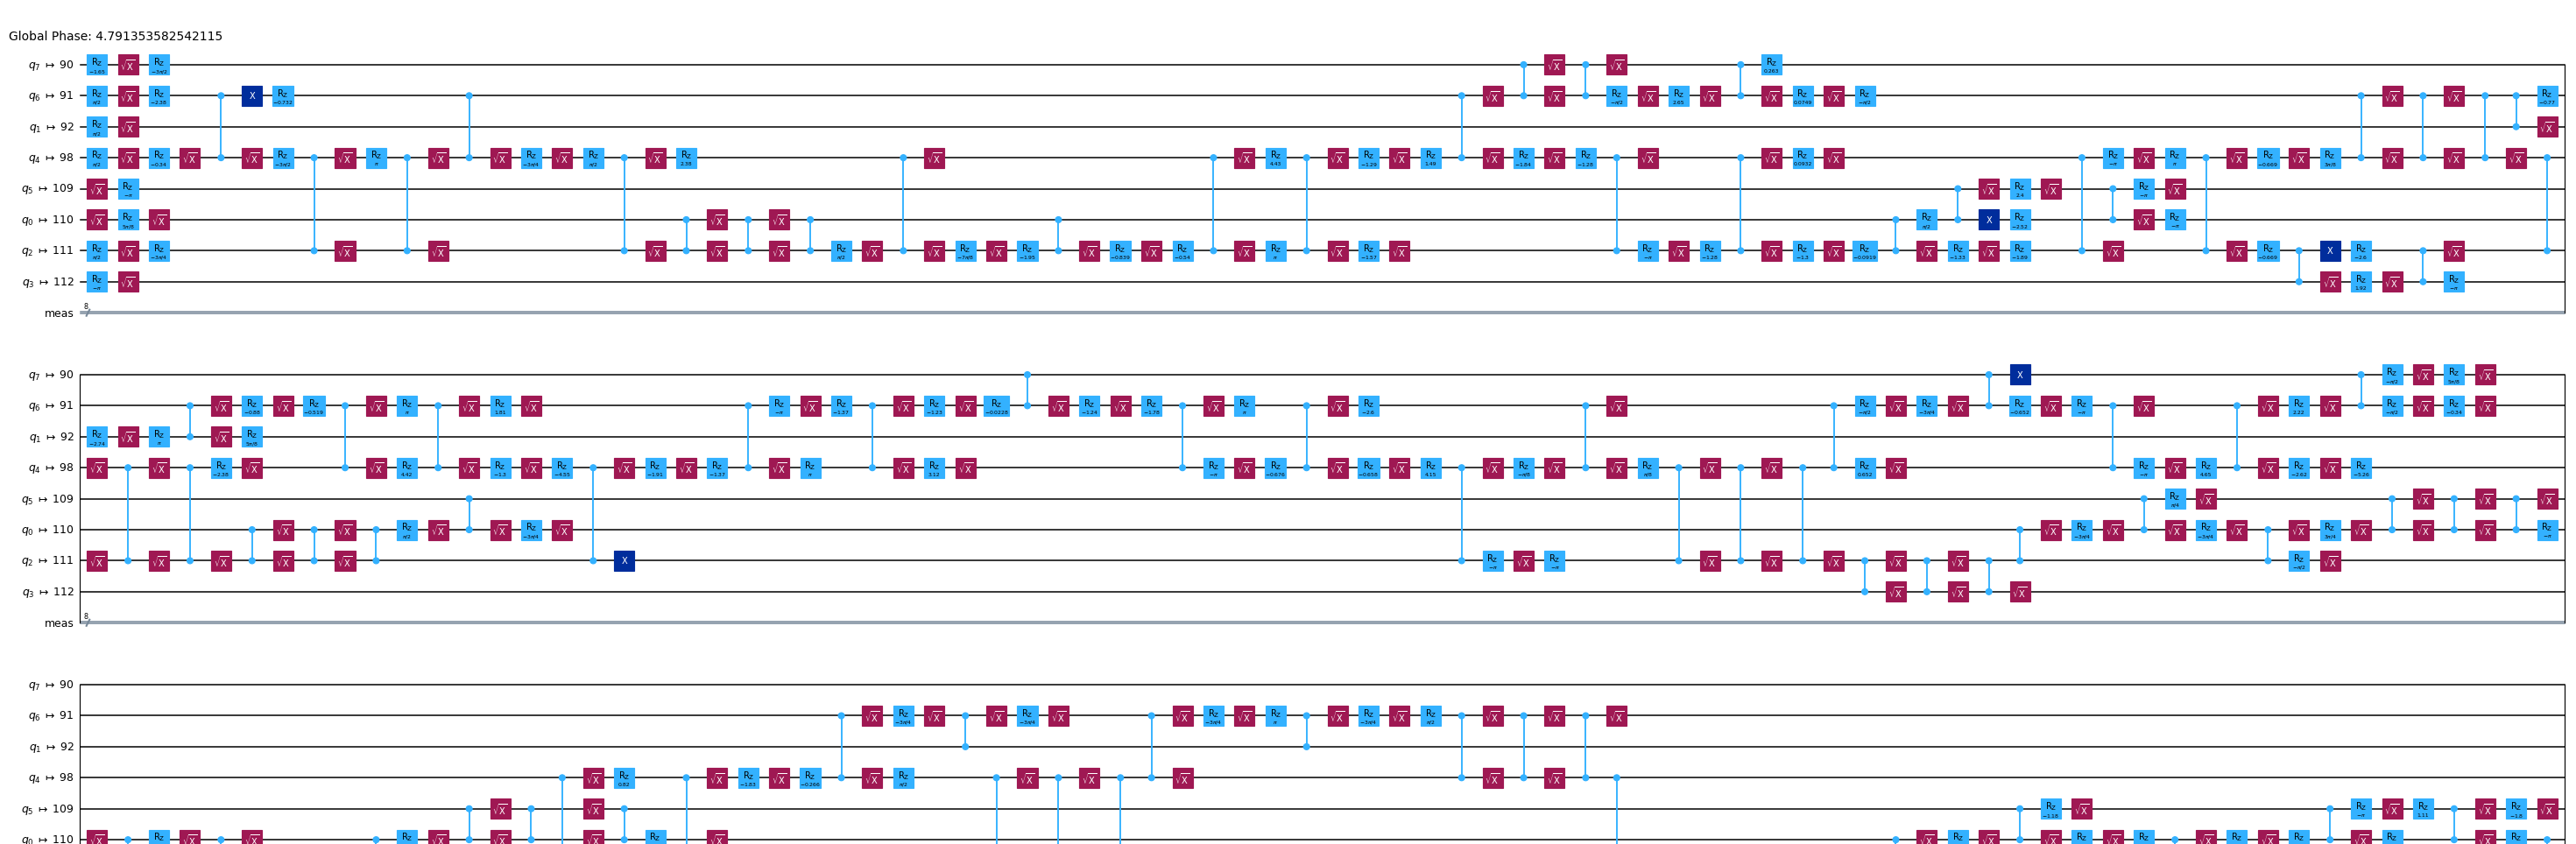
\includegraphics[width=0.98\linewidth,height=0.80\textheight,keepaspectratio]{gm_qaoa_transpiled_folded_part_1.png}
\caption{\GMQAOA{} $p=1$ transpiled circuit, folded-view panel 1 of 4.}
\end{figure}
\end{landscape}

\begin{landscape}
\begin{figure}[H]
\centering
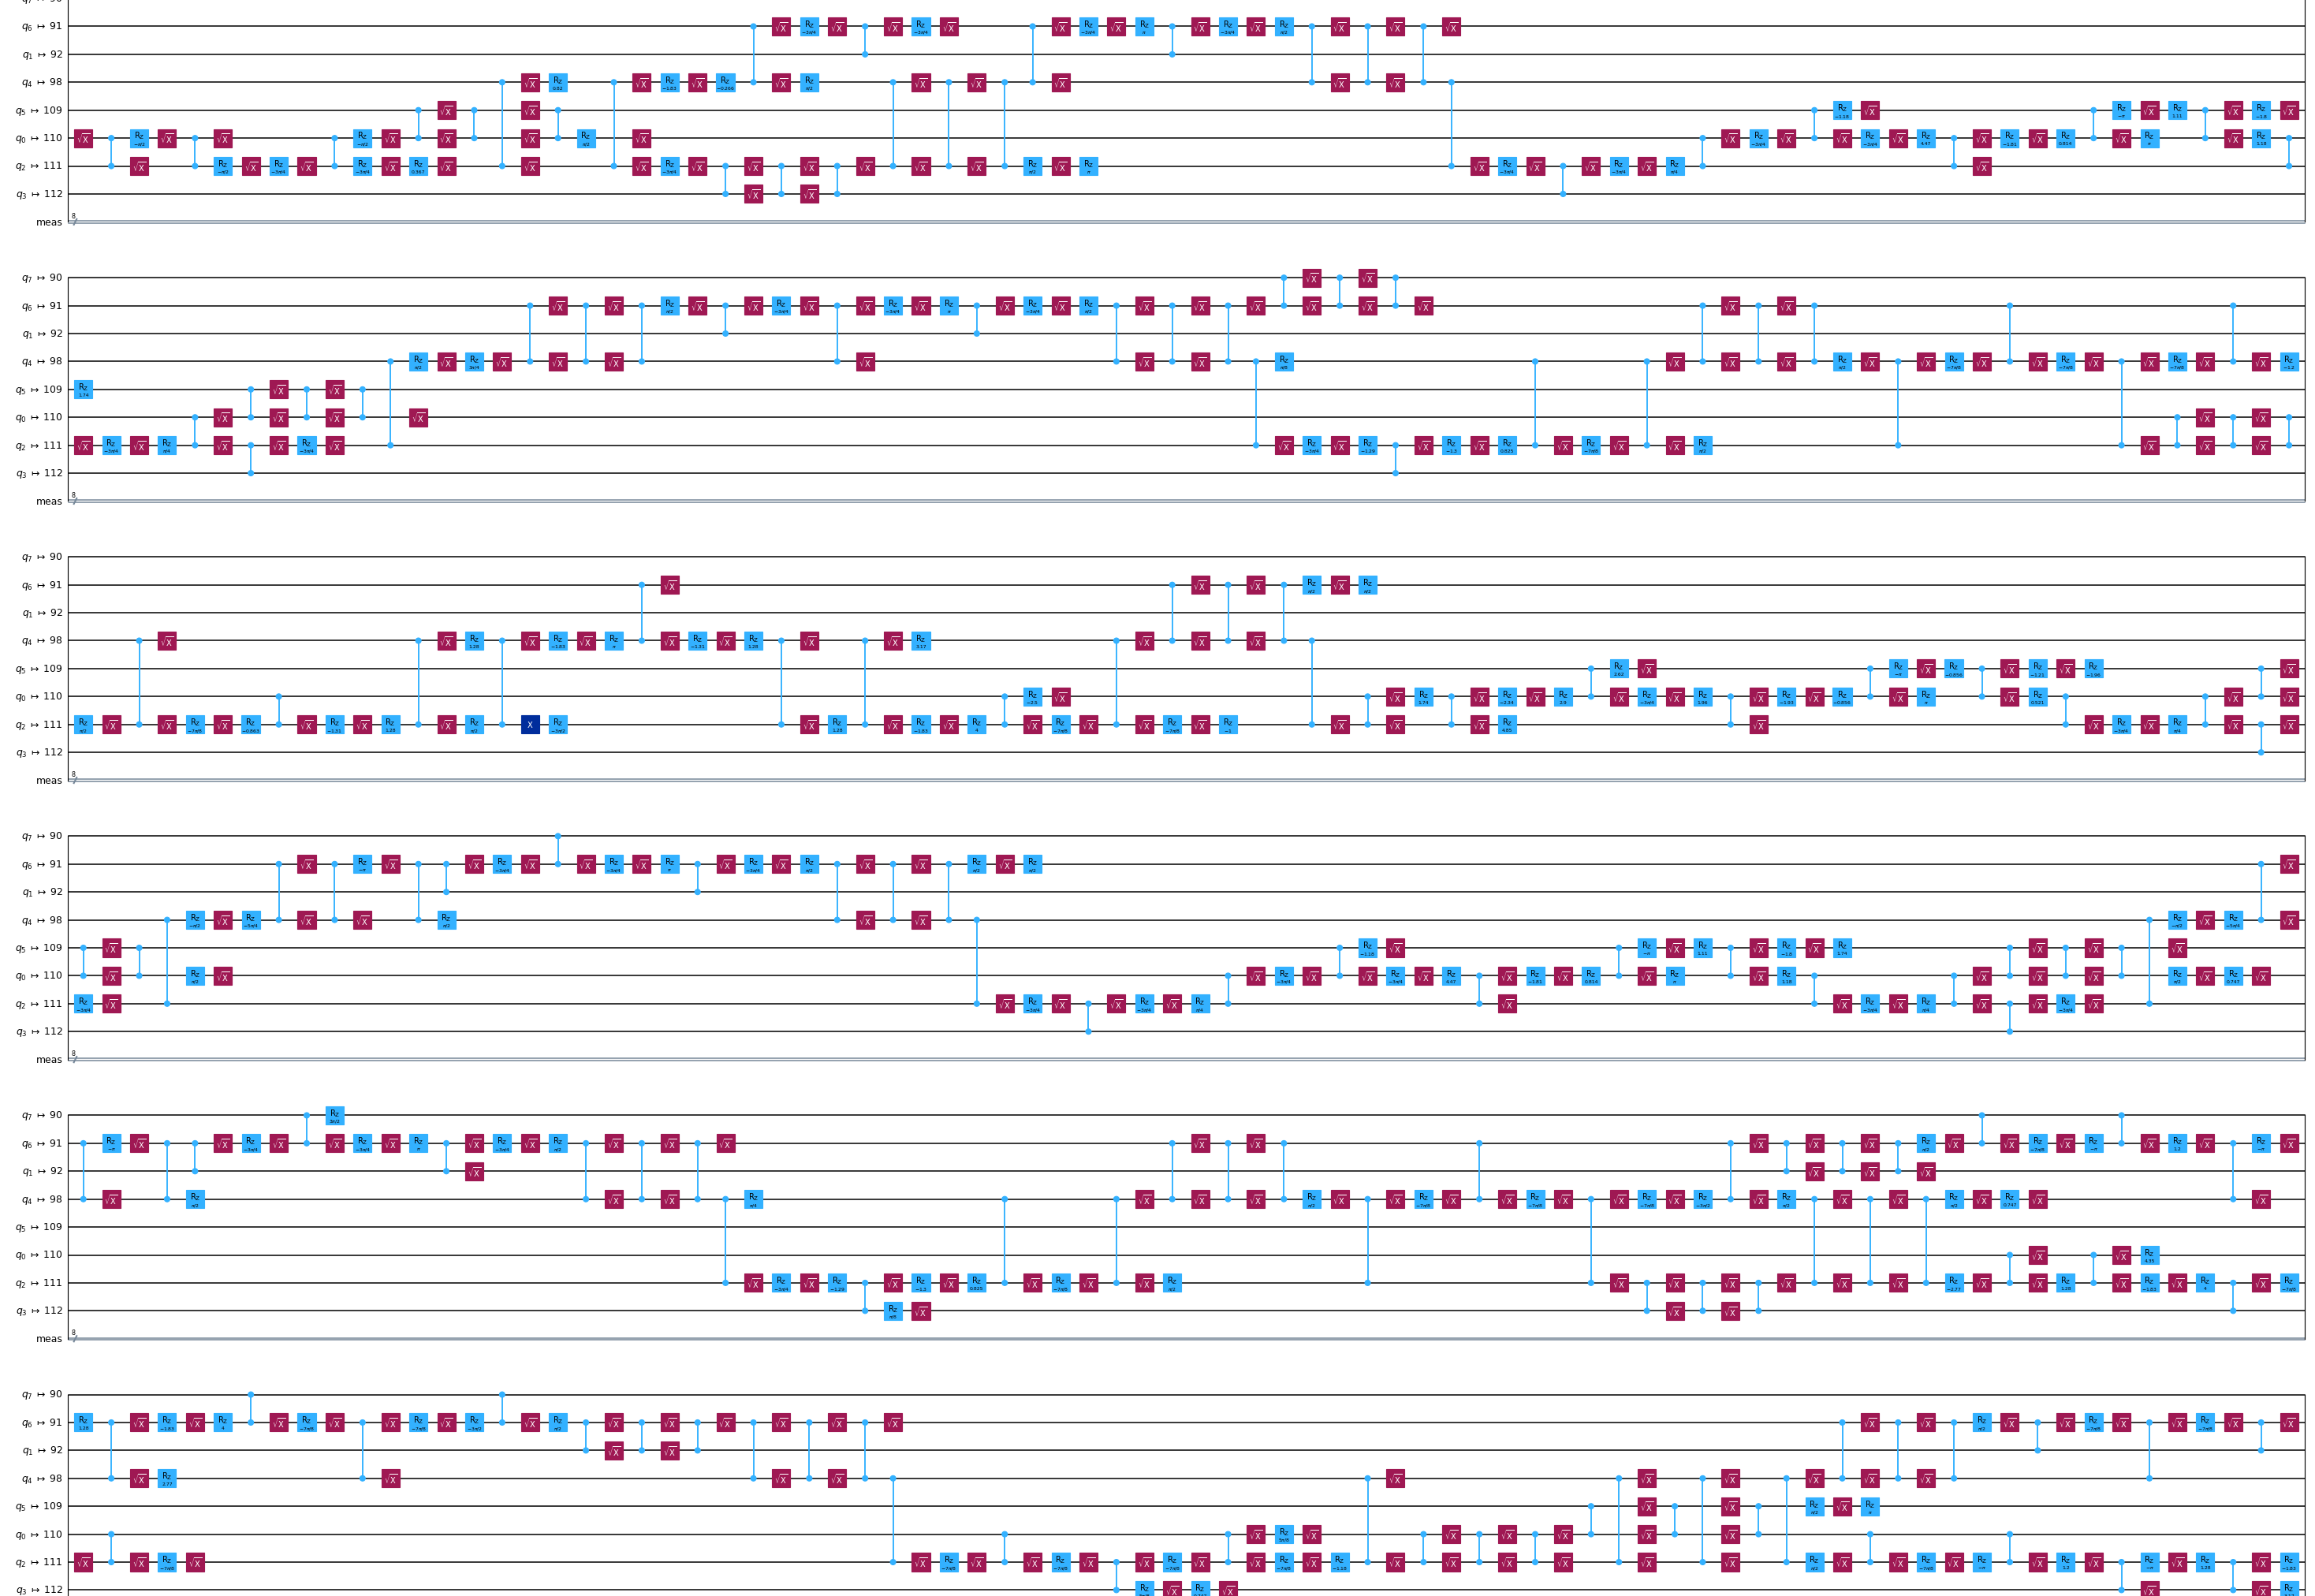
\includegraphics[width=0.98\linewidth,height=0.80\textheight,keepaspectratio]{gm_qaoa_transpiled_folded_part_2.png}
\caption{\GMQAOA{} $p=1$ transpiled circuit, folded-view panel 2 of 4.}
\end{figure}
\end{landscape}

\begin{landscape}
\begin{figure}[H]
\centering
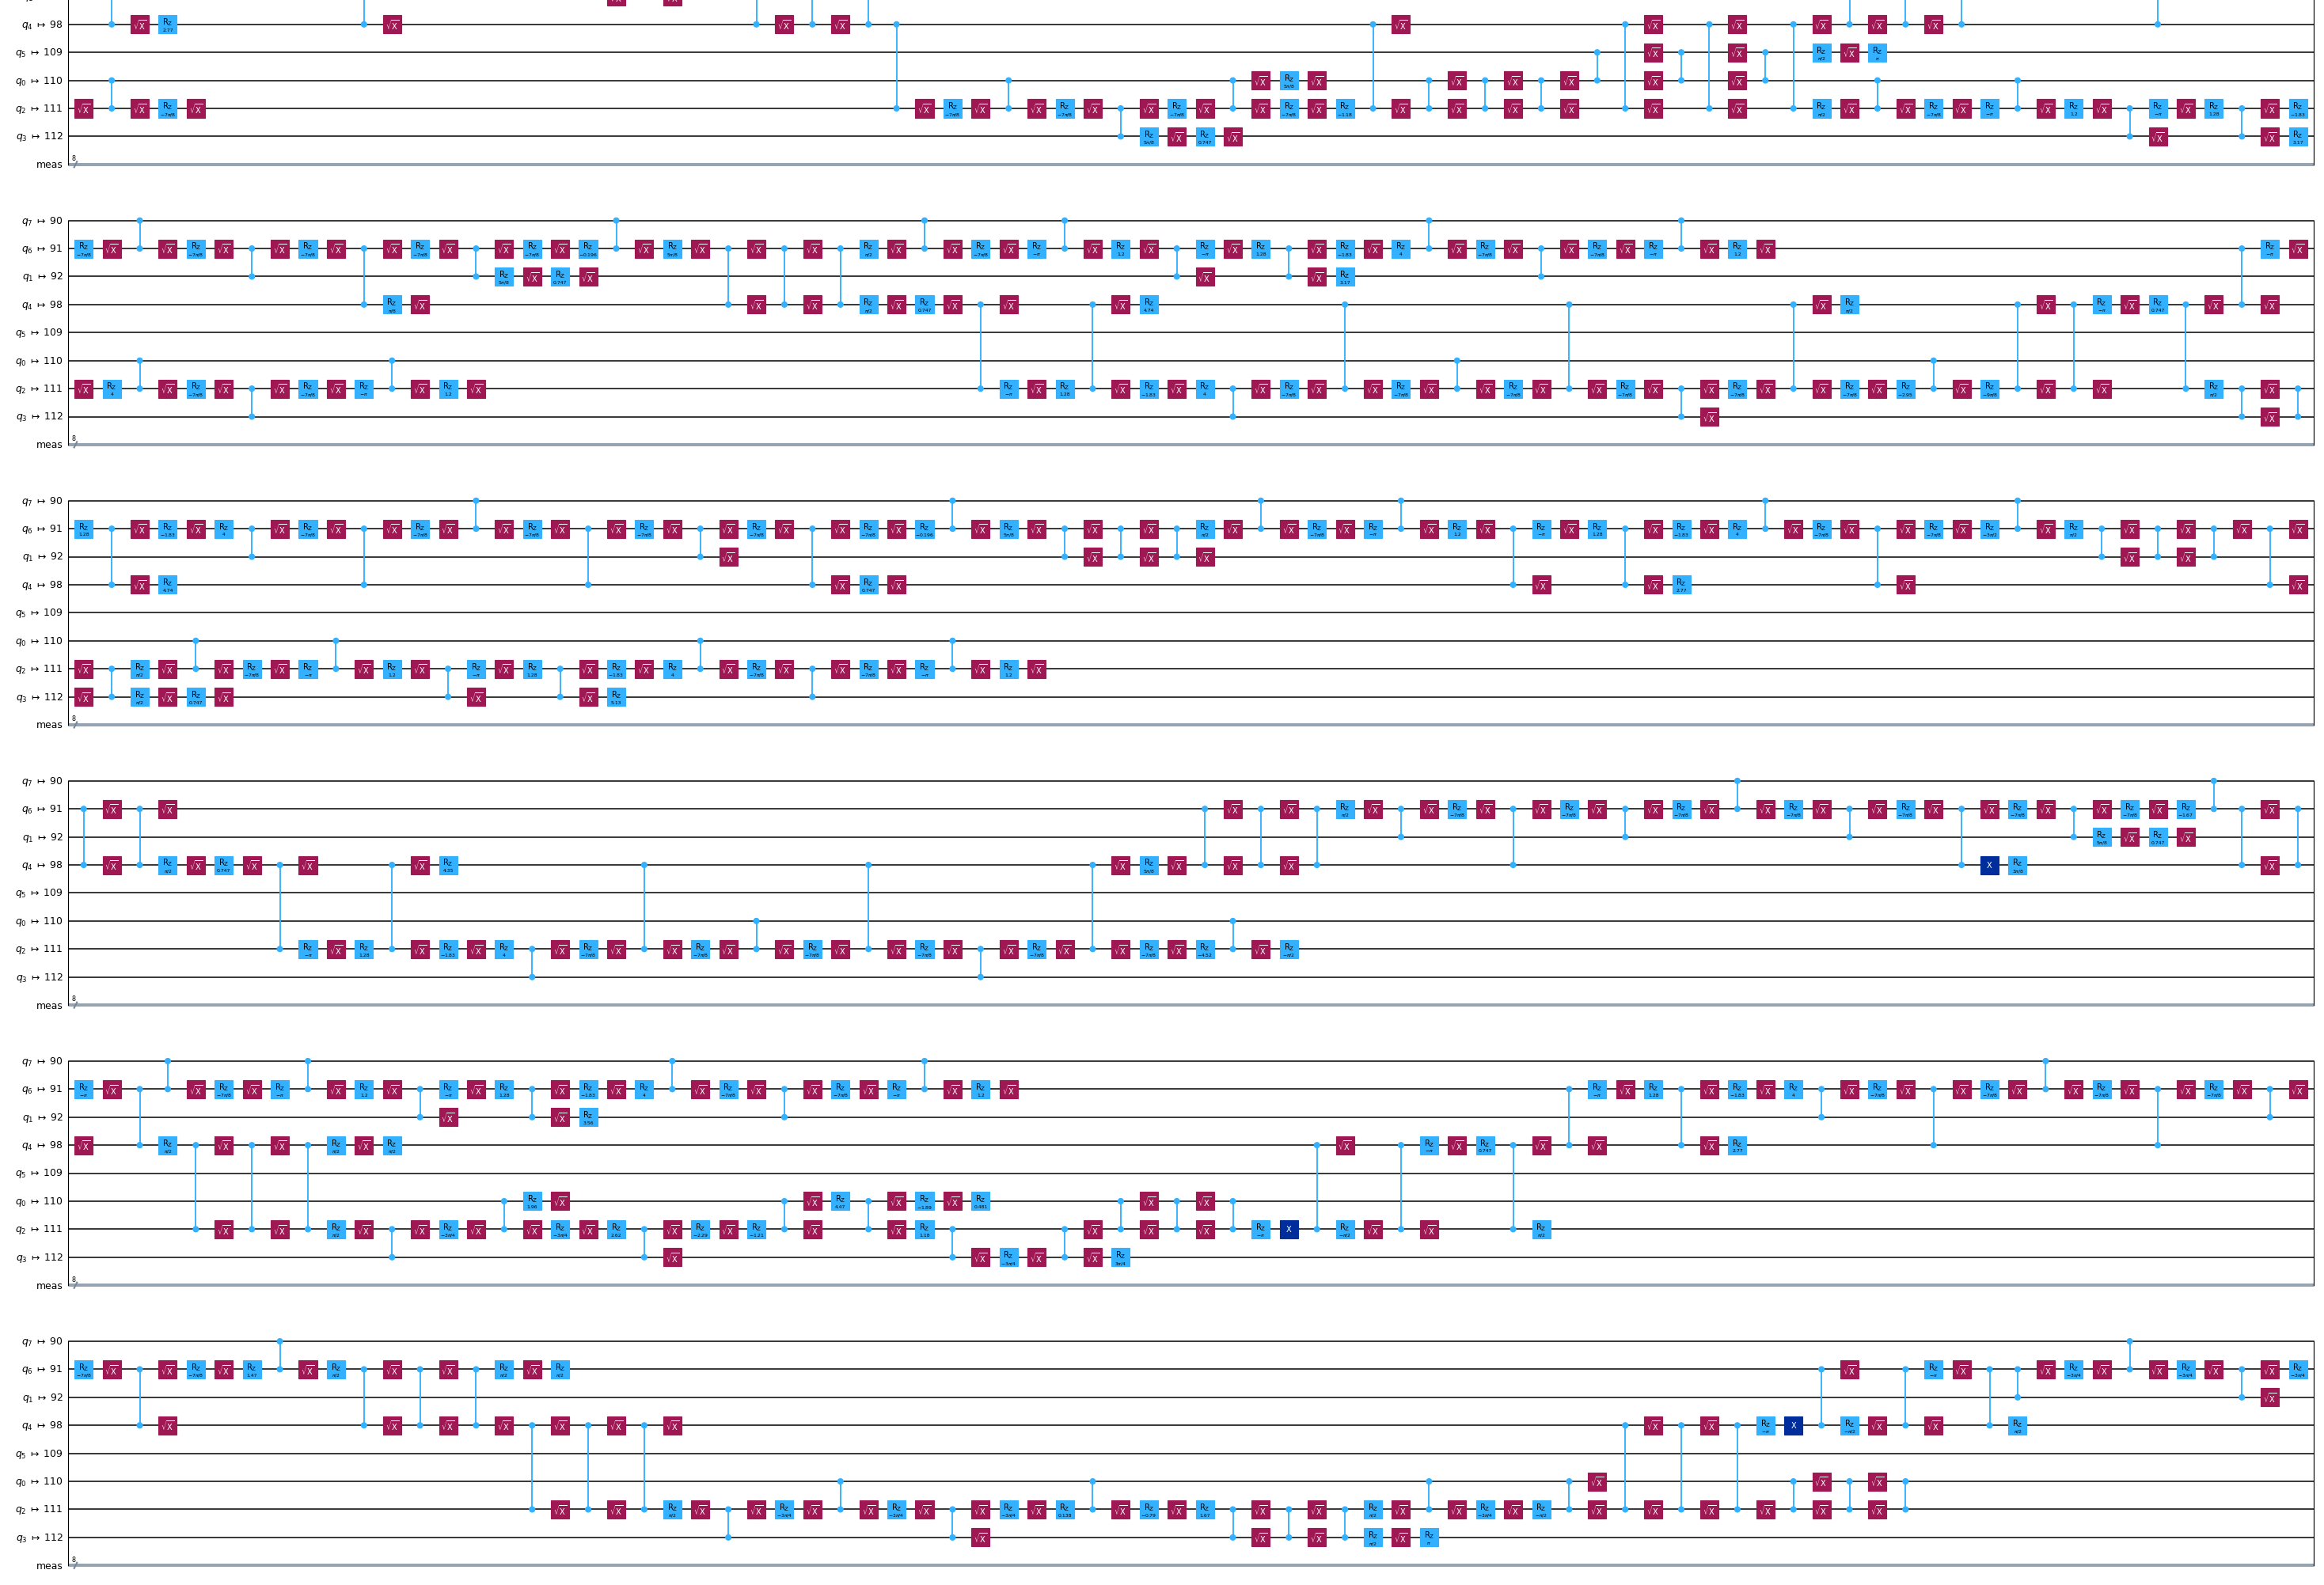
\includegraphics[width=0.98\linewidth,height=0.80\textheight,keepaspectratio]{gm_qaoa_transpiled_folded_part_3.png}
\caption{\GMQAOA{} $p=1$ transpiled circuit, folded-view panel 3 of 4.}
\end{figure}
\end{landscape}

\begin{landscape}
\begin{figure}[H]
\centering
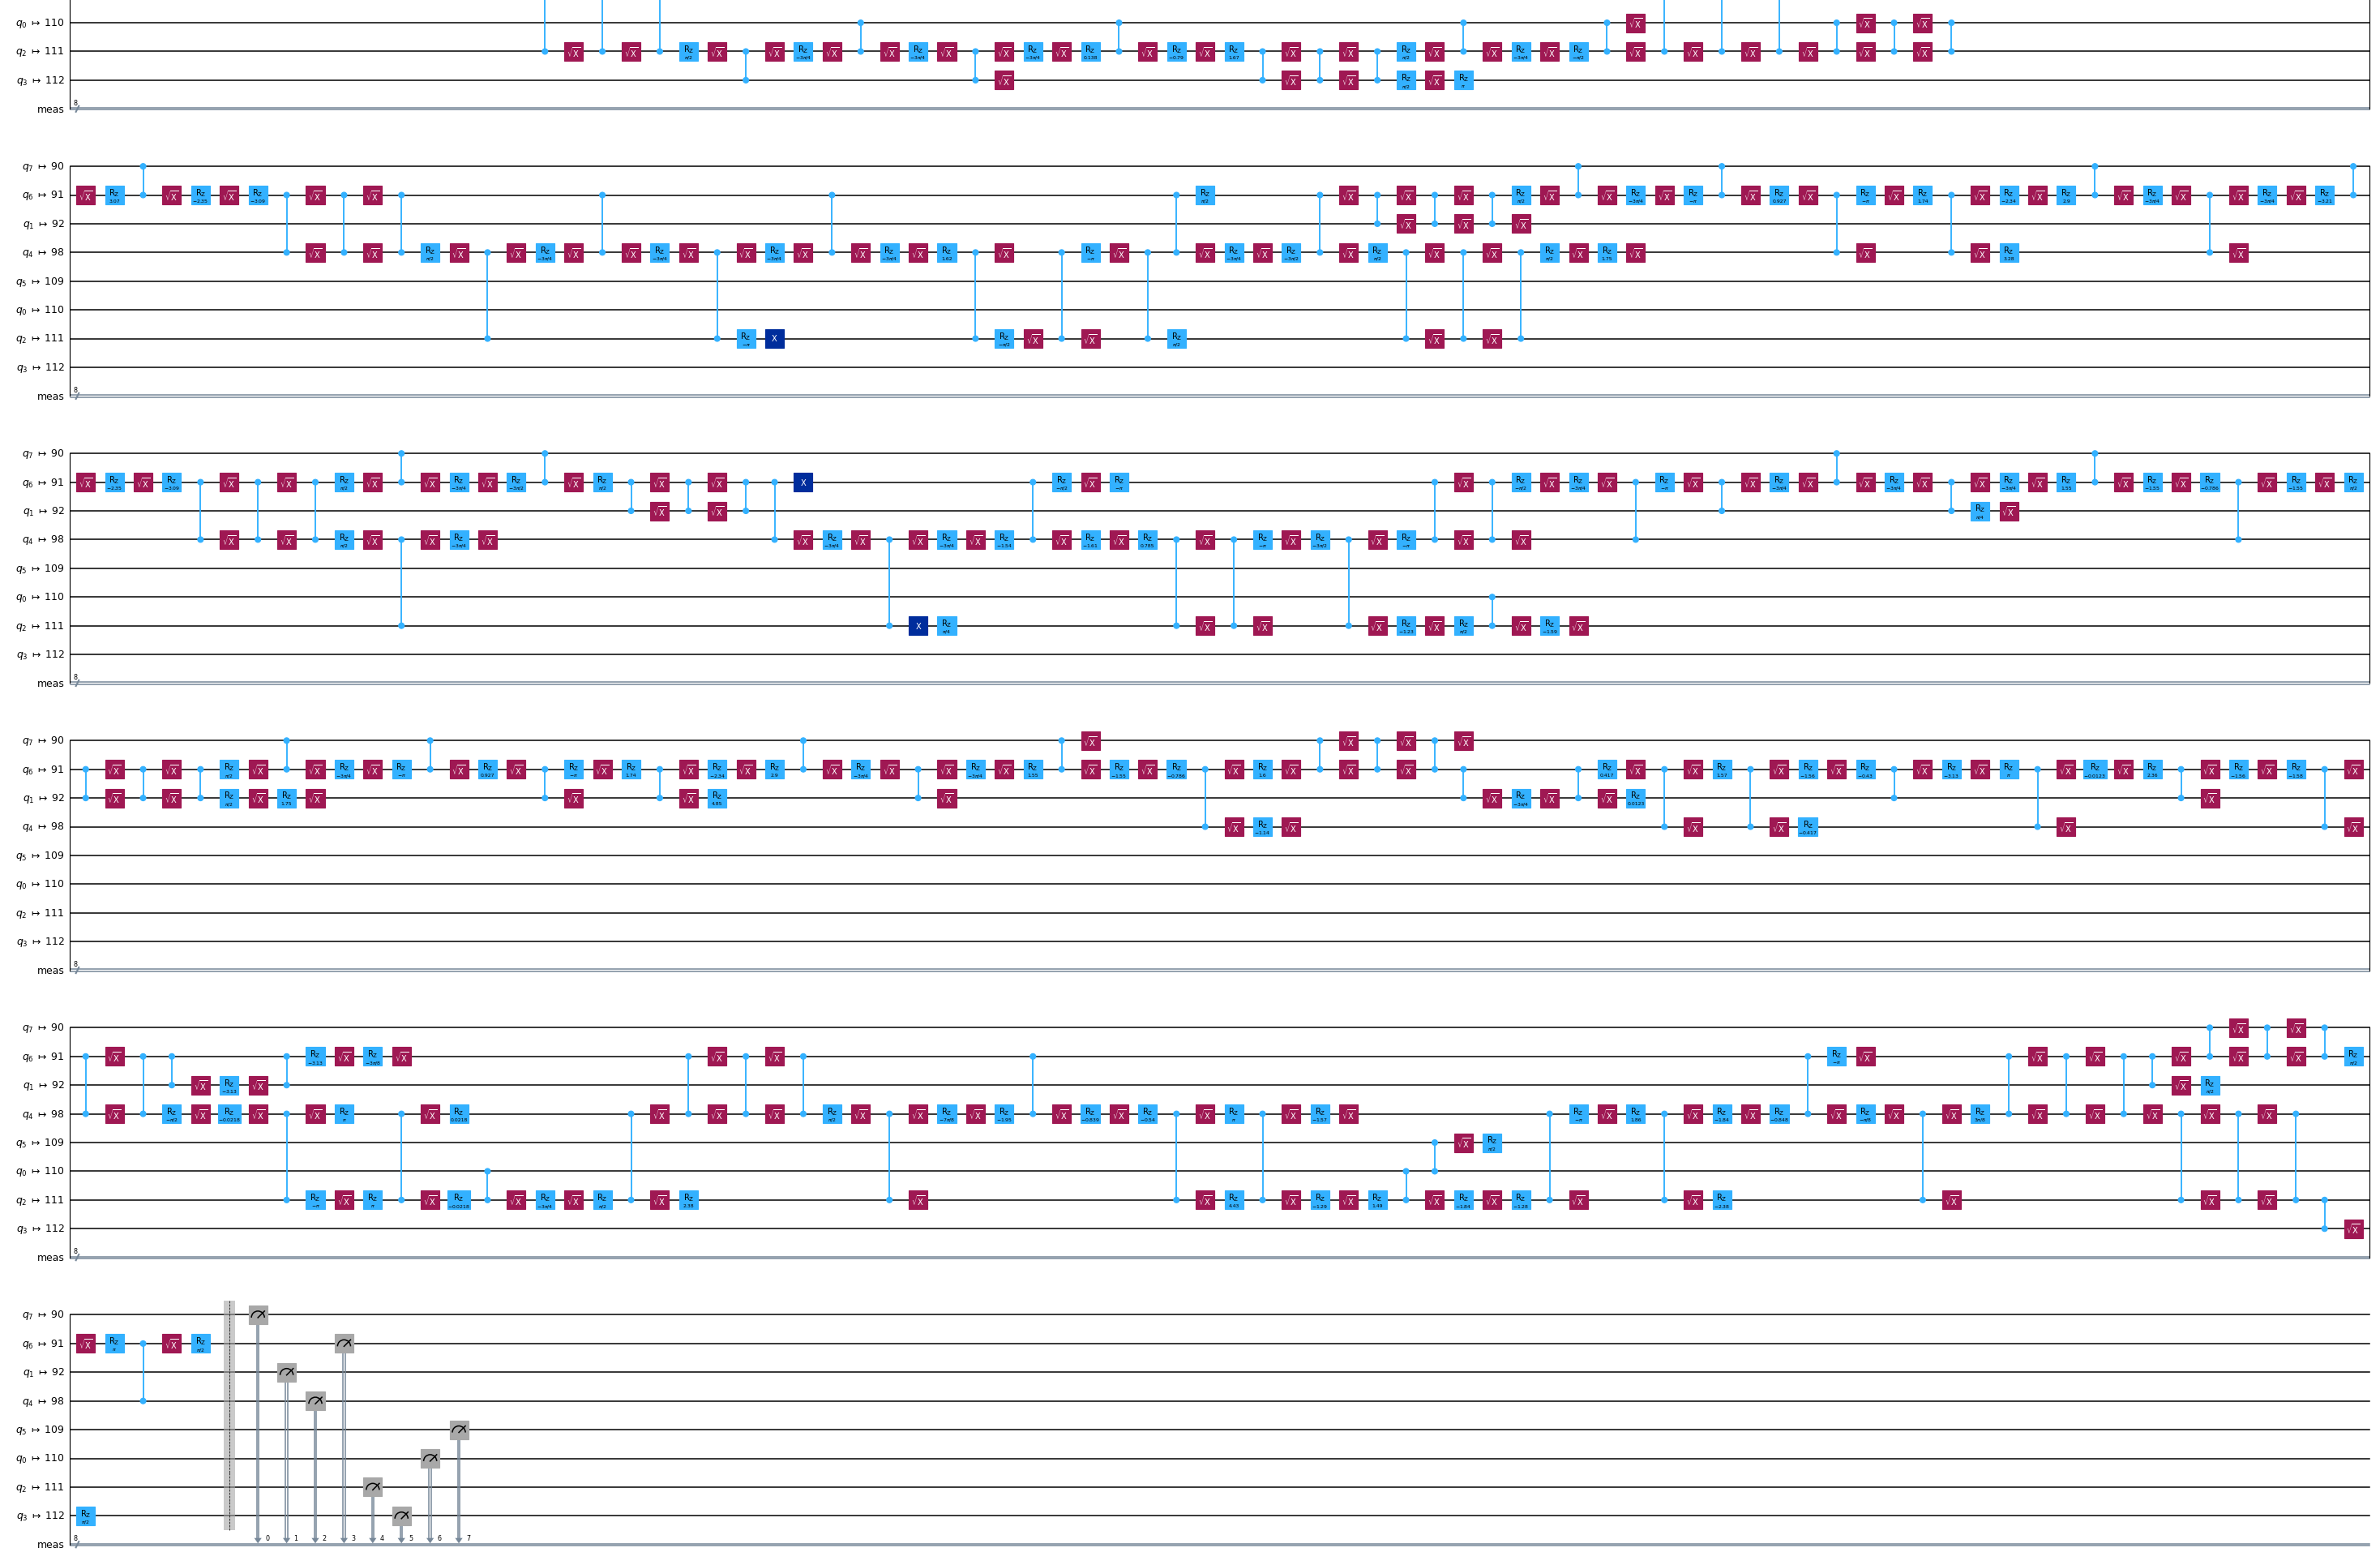
\includegraphics[width=0.98\linewidth,height=0.80\textheight,keepaspectratio]{gm_qaoa_transpiled_folded_part_4.png}
\caption{\GMQAOA{} $p=1$ transpiled circuit, folded-view panel 4 of 4.}
\end{figure}
\end{landscape}


\section{Hardware Distribution Detail}
\label{app:distributions}

\subsection{Feasible-state counts}

\begin{table}[H]
\centering
\caption{Complete counts on the six feasible states of the $4\times2$ problem.}
\small
\begin{tabular}{lrr|rr|r}
\toprule
 & \multicolumn{2}{c}{Standard \QAOA{}} & \multicolumn{2}{c}{\GMQAOA{}} & \\
Bitstring & Count & Ideal probability & Count & Ideal probability & Score\\
\midrule
\texttt{10011001} & 16 & 0.023380 & 29 & 0.503666 & 3.25\\
\texttt{10100101} & 15 & 0.016493 & 24 & 0.195717 & 2.60\\
\texttt{01101001} & 15 & 0.016240 & 10 & 0.174404 & 2.55\\
\texttt{10010110} & 11 & 0.013311 & 24 & 0.054315 & 2.20\\
\texttt{01011010} & 12 & 0.013112 & 21 & 0.042262 & 2.15\\
\texttt{01100110} & 10 & 0.009046 & 14 & 0.029636 & 1.50\\
\midrule
Total feasible & 79 & 0.091582 & 122 & 1.000000 & --\\
\bottomrule
\end{tabular}
\end{table}

\subsection{Most frequent outcomes}

\begin{table}[H]
\centering
\caption{Ten most frequent outcomes per hardware circuit.}
\scriptsize
\begin{tabular}{llrrrrl}
\toprule
Algorithm & Bitstring & Count & Observed $q(x)$ & Ideal $p(x)$ & Score & Feasible\\
\midrule
Standard & \texttt{10101101} & 23 & 0.022461 & 0.019028 & 3.50 & No\\
Standard & \texttt{10100111} & 18 & 0.017578 & 0.014731 & 2.90 & No\\
Standard & \texttt{10110101} & 17 & 0.016602 & 0.015252 & 3.30 & No\\
Standard & \texttt{10111001} & 16 & 0.015625 & 0.019959 & 3.80 & No\\
Standard & \texttt{10011001} & 16 & 0.015625 & 0.023380 & 3.25 & Yes\\
Standard & \texttt{10011110} & 15 & 0.014648 & 0.016861 & 3.10 & No\\
Standard & \texttt{01101001} & 15 & 0.014648 & 0.016240 & 2.55 & Yes\\
Standard & \texttt{10100101} & 15 & 0.014648 & 0.016493 & 2.60 & Yes\\
Standard & \texttt{10011101} & 14 & 0.013672 & 0.016719 & 3.65 & No\\
Standard & \texttt{10011011} & 13 & 0.012695 & 0.017883 & 3.55 & No\\
\midrule
GM & \texttt{10011001} & 29 & 0.028320 & 0.503666 & 3.25 & Yes\\
GM & \texttt{10010110} & 24 & 0.023438 & 0.054315 & 2.20 & Yes\\
GM & \texttt{10100101} & 24 & 0.023438 & 0.195717 & 2.60 & Yes\\
GM & \texttt{01011010} & 21 & 0.020508 & 0.042262 & 2.15 & Yes\\
GM & \texttt{01000110} & 16 & 0.015625 & 0.000000 & 0.95 & No\\
GM & \texttt{00100101} & 14 & 0.013672 & 0.000000 & 1.80 & No\\
GM & \texttt{01010010} & 14 & 0.013672 & 0.000000 & 1.25 & No\\
GM & \texttt{01100110} & 14 & 0.013672 & 0.029636 & 1.50 & Yes\\
GM & \texttt{10010001} & 13 & 0.012695 & 0.000000 & 2.35 & No\\
GM & \texttt{10011010} & 13 & 0.012695 & 0.000000 & 2.70 & No\\
\bottomrule
\end{tabular}
\end{table}

The complete 512-row-by-two-algorithm table is supplied as a CSV rather than reproduced in full in the PDF.

\section{Reproducibility Metadata and Claims Boundary}
\label{app:reproducibility}

\subsection{Repository artifact}

The source repository contains:
\begin{verbatim}
QI26-20-QUBO-QAOA-Benchmark/
|-- README.md
|-- requirements.txt
|-- QI26_20_QUBO_QAOA_GM_QAOA_Benchmark.ipynb
|-- results/
`-- paper/
\end{verbatim}
The manuscript PDF is intended for the repository path
\begin{verbatim}
paper/QI26_20_preprint.pdf
\end{verbatim}

\subsection{Core run parameters}

\begin{table}[H]
\centering
\caption{Core reproducibility parameters.}
\begin{tabular}{ll}
\toprule
Parameter & Value\\
\midrule
Data / transpiler / simulator seed & 2026\\
Standard depths & $p\in\{1,2,3\}$ ideal; $p=1$ hardware\\
GM depth & $p=1$\\
Optimizer & COBYLA\\
Ideal candidate shots & 4096\\
Hardware shots & 1024 per circuit\\
Hardware instance & $4\times2$, exact capacities $[2,2]$\\
Backend & \texttt{ibm\_marrakesh}\\
Optimization level & 3\\
Dynamical decoupling & XpXm\\
Gate twirling & Enabled\\
Job ID & \texttt{d9vl8qfo3ppc73akfak0}\\
\bottomrule
\end{tabular}
\end{table}

\subsection{Supported and unsupported statements}

\begin{table}[H]
\centering
\small
\begin{tabularx}{\textwidth}{>{\raggedright\arraybackslash}X>{\raggedright\arraybackslash}X}
\toprule
Supported by the artifact & Not supported by the artifact\\
\midrule
One-to-one and fixed exact-capacity \QUBO{} models are implemented and validated. & The implementation supports arbitrary dynamic capacities without extension.\\
Standard \QAOA{} is compared at $p=1,2,3$ in ideal simulation. & Standard \QAOA{} was run on hardware at all three depths.\\
The fixed \GMQAOA{} circuits preserve the feasible subspace ideally. & The QPU preserves the \GMQAOA{} feasible subspace.\\
Both physical circuits sampled the exact optimum. & Either algorithm finds the optimum with high probability.\\
The operational Grover mixer matches the equations in Bärtschi--Eidenbenz. & The general $O(n^3)$ state-preparation construction is reproduced.\\
The recorded \GMQAOA{} circuit has substantially higher depth and CZ count. & The same ratio holds for all devices and instances.\\
No quantum advantage is established. & The data establish or refute quantum advantage in general.\\
\bottomrule
\end{tabularx}
\end{table}

\subsection{Credential hygiene}

No IBM Quantum credential is required to inspect or reproduce the archived analysis. Any future execution should obtain the token from a Colab secret or environment variable and must not commit the token to the repository.


\clearpage
\bibliographystyle{unsrt}
\bibliography{references}

\end{document}
